% * ANEXO A *
\chapter{Capturas de la Interfaz de Usuario} \label{ch:anexoA}

\section{Interfaz de Estadísticas}

Cada una de las estadísticas ha sido diseñada de manera independiente y autocontenida. Es por esto por lo que, aunque se sigan las directrices de diseño generales de la página, cada una tiene un caracter y presentación diferenciable. También cabe destacar que, en algunas de ellas, se ha preferido desarrollar la implementación funcional de manera más robusta, antes de invertir el tiempo en mejorar por completo la estética de la presentación.

\begin{figure}[H]
  \centering
  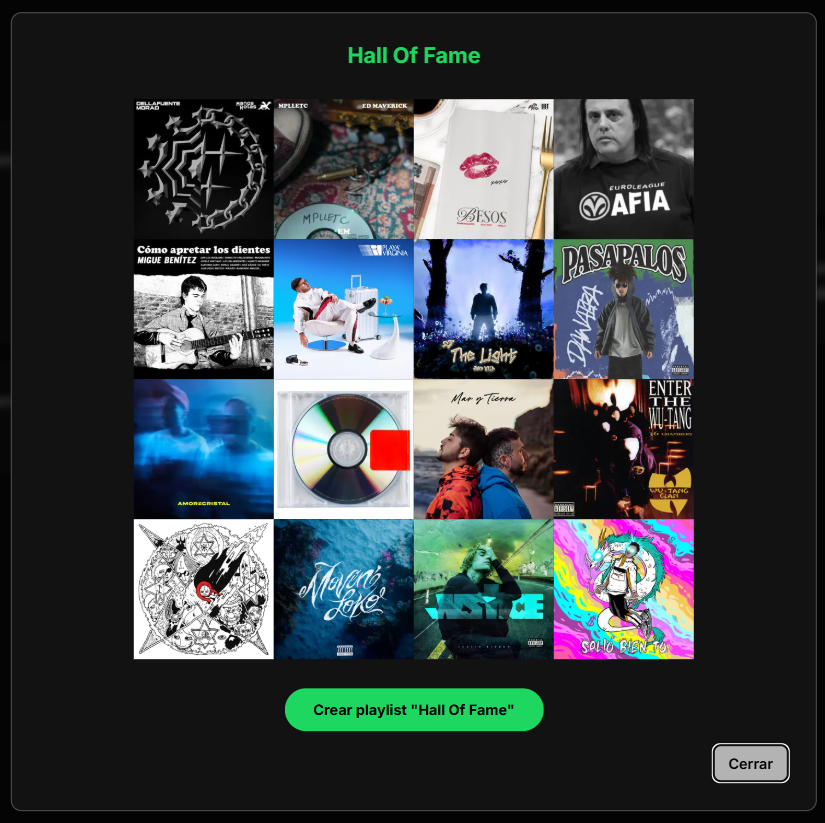
\includegraphics[width=0.45\textwidth]{figures/capturas_ui/hall_of_fame.png}
  \caption{Interfaz de la estadística \textit{Hall Of Fame}.}
  \label{fig:hall_of_fame}
\end{figure}

\begin{figure}[H]
  \centering
  \vspace{-10pt}
  \begin{minipage}{0.32\textwidth}
    \centering
    \includegraphics[width=\textwidth]{figures/capturas_ui/la_bitacora_año.png}
    \caption{Interfaz de la estadística \textit{La Bitácora} (año).}
    \label{fig:la_bitacora_año}
  \end{minipage}
  \begin{minipage}{0.32\textwidth}
    \centering
    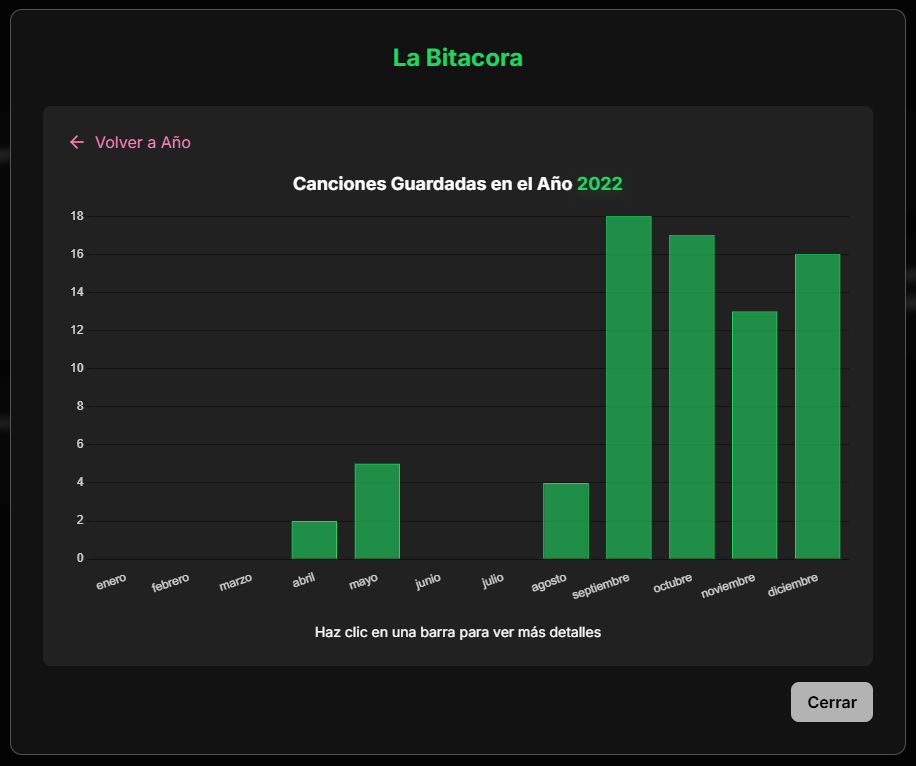
\includegraphics[width=\textwidth]{figures/capturas_ui/la_bitacora_mes.png}
    \caption{Interfaz de la estadística \textit{La Bitácora} (mes).}
    \label{fig:la_bitacora_mes}
  \end{minipage}
  \begin{minipage}{0.32\textwidth}
    \centering
    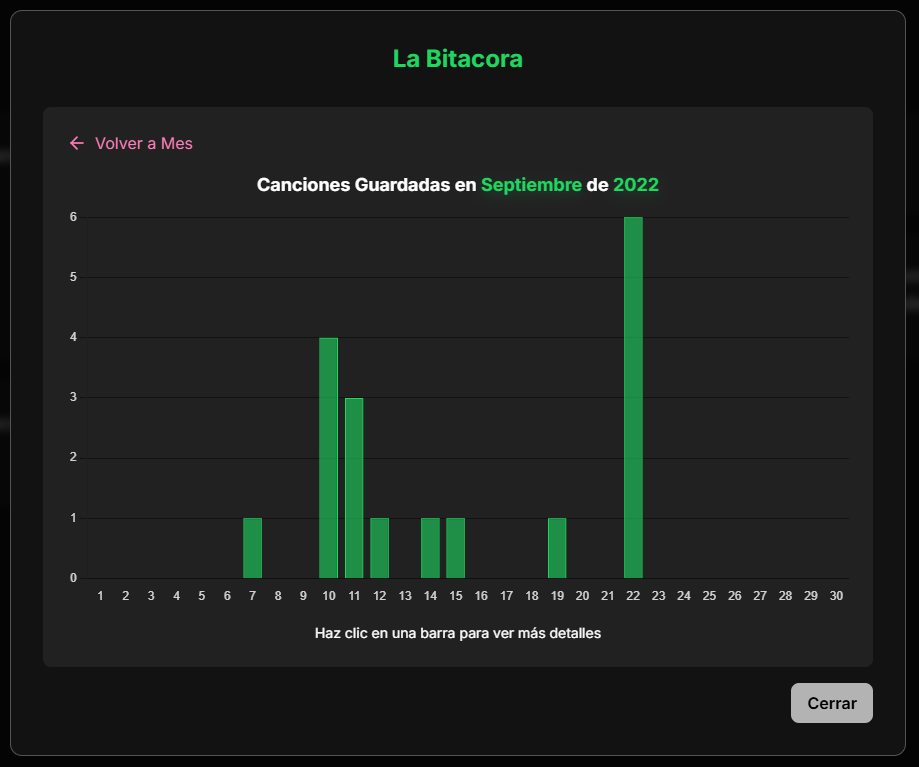
\includegraphics[width=\textwidth]{figures/capturas_ui/la_bitacora_dia.png}
    \caption{Interfaz de la estadística \textit{La Bitácora} (día).}
    \label{fig:la_bitacora_dia}
  \end{minipage}
  \caption{Interfaz de la estadística \textit{La Bitácora}, en los tres diferentes niveles de detalle.}
  \label{fig:la_bitacora}
\end{figure}

\begin{figure}[H]
  \centering
  \vspace{-10pt}
  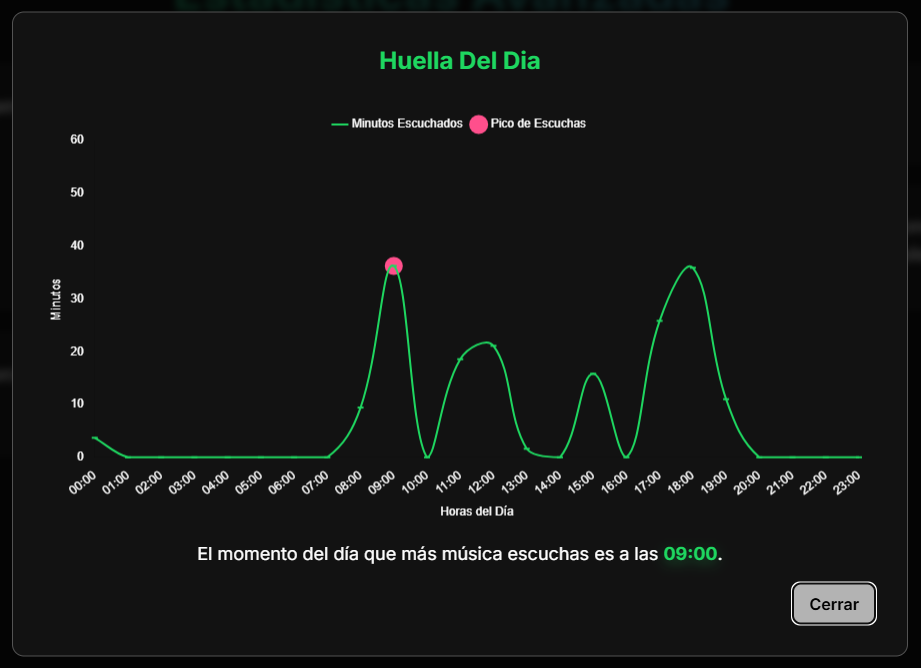
\includegraphics[width=0.55\textwidth]{figures/capturas_ui/huella_del_dia.png}
  \caption{Interfaz de la estadística \textit{Huella Del Día}.}
  \label{fig:huella_del_dia}
\end{figure}

\begin{figure}[H]
  \centering
  \vspace{-10pt}
  \begin{minipage}{0.47\textwidth}
    \centering
    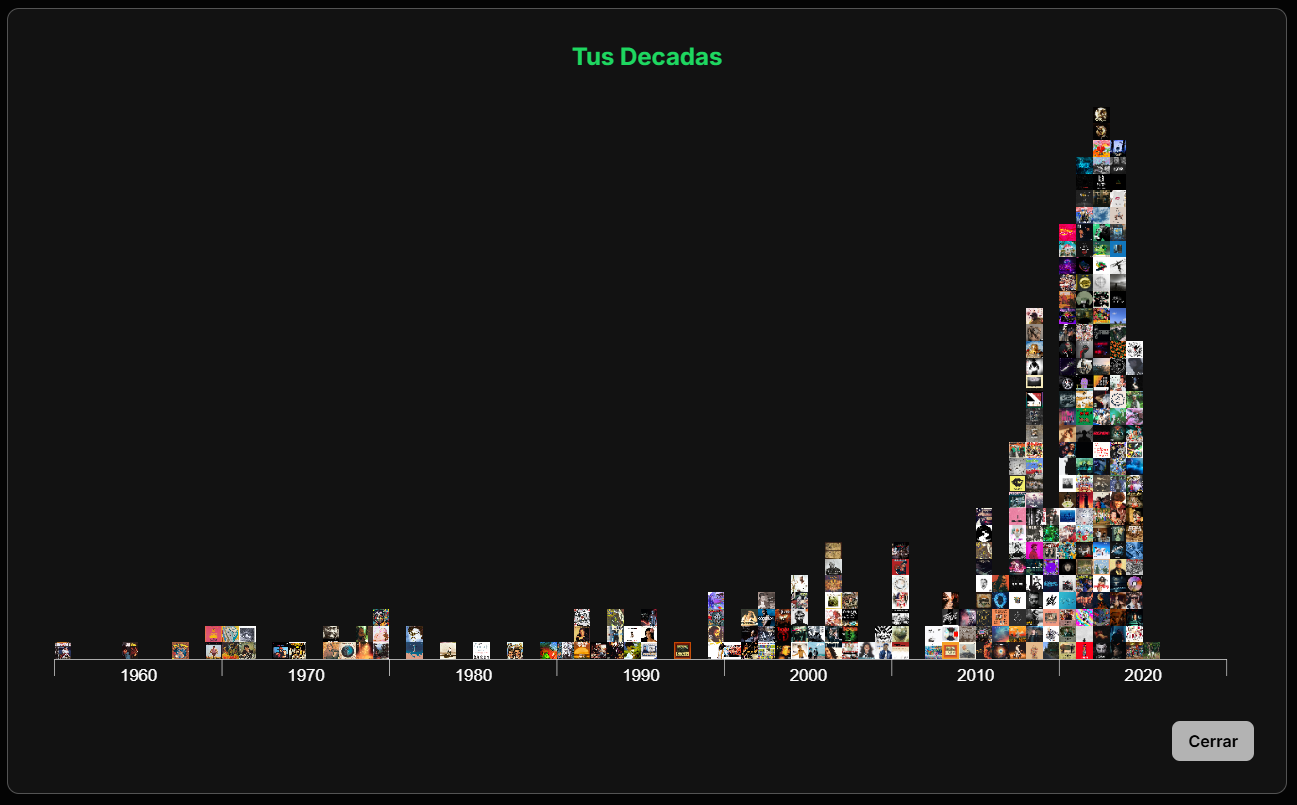
\includegraphics[width=\textwidth]{figures/capturas_ui/tus_decadas_out.png}
    \caption{Interfaz de la estadística \textit{Tus Décadas} (zoom out).}
    \label{fig:tus_decadas_out}
  \end{minipage}
  \begin{minipage}{0.47\textwidth}
    \centering
    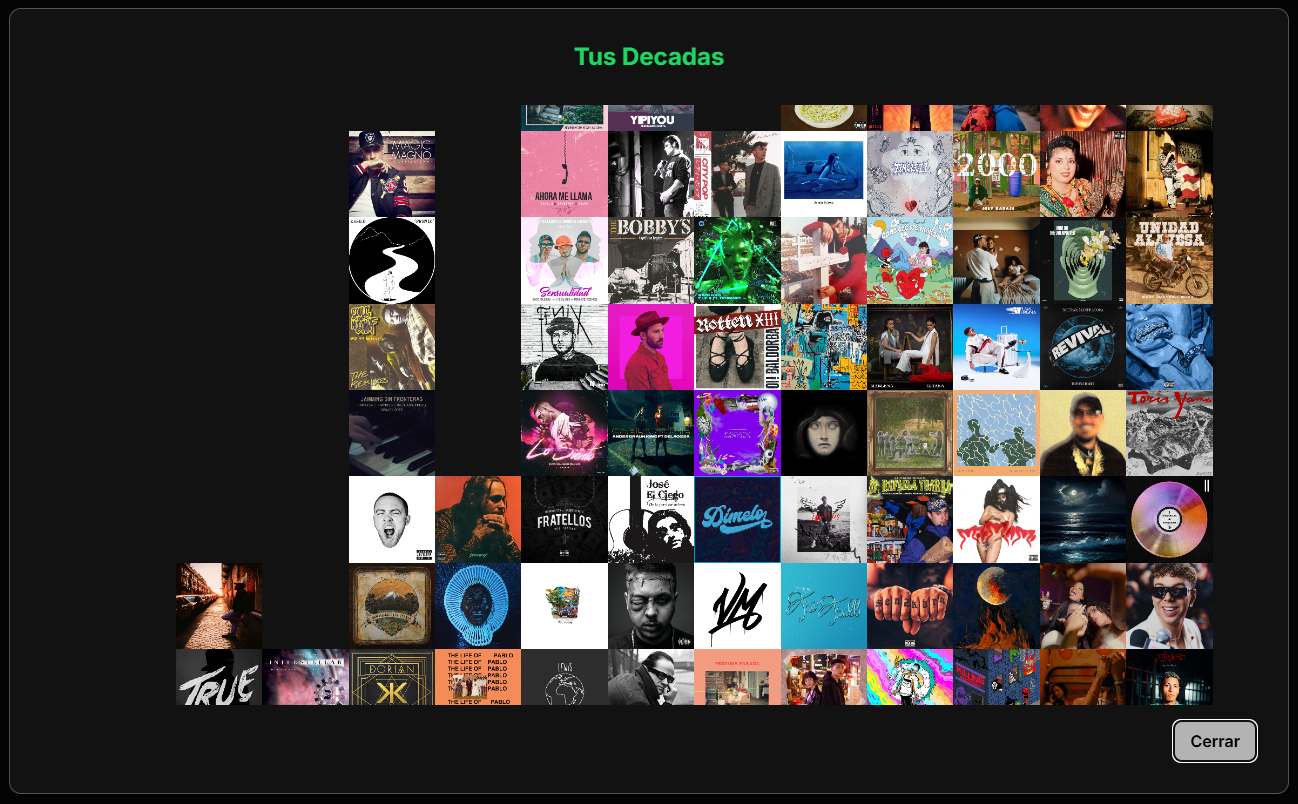
\includegraphics[width=\textwidth]{figures/capturas_ui/tus_decadas_zoom.png}
    \caption{Interfaz de la estadística \textit{Tus Décadas} (zoom in).}
    \label{fig:tus_decadas_zoom}
  \end{minipage}
  \caption{Interfaz de la estadística \textit{Tus Décadas}, en diferentes niveles de zoom.}
  \label{fig:tus_decadas}
\end{figure}

\begin{figure}[H]
  \centering
  \vspace{-10pt}
  \begin{minipage}{0.47\textwidth}
    \centering
    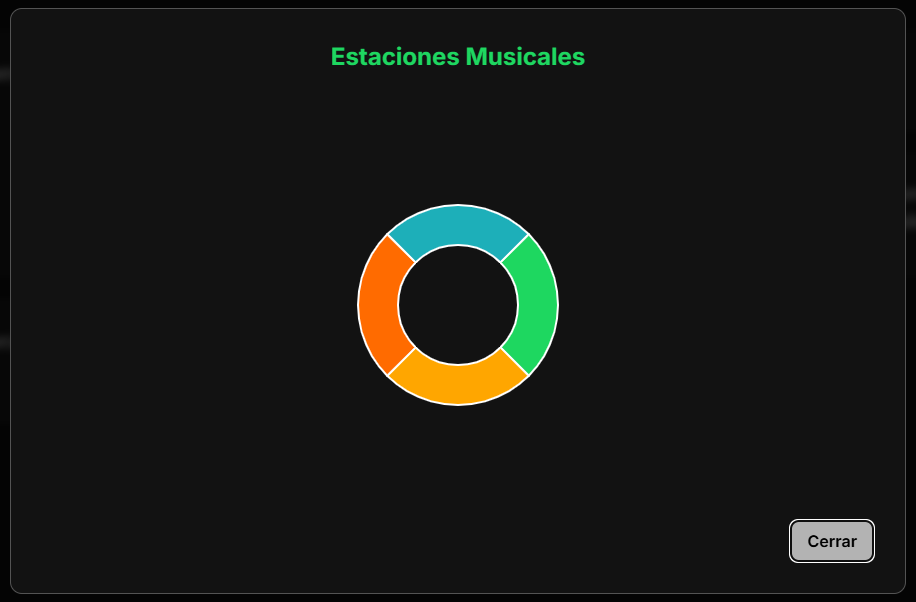
\includegraphics[width=\textwidth]{figures/capturas_ui/estaciones_musicales_cerrado.png}
    \caption{Interfaz de la estadística \textit{Estaciones Musicales} (cerrado).}
    \label{fig:estaciones_musicales_cerrado}
  \end{minipage}
  \begin{minipage}{0.47\textwidth}
    \centering
    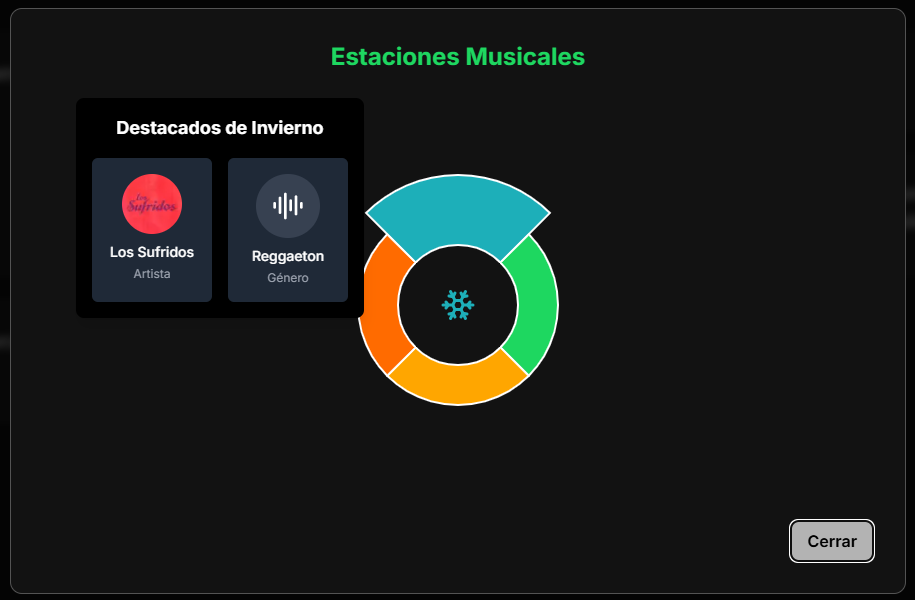
\includegraphics[width=\textwidth]{figures/capturas_ui/estaciones_musicales_abierto.png}
    \caption{Interfaz de la estadística \textit{Estaciones Musicales} (abierto).}
    \label{fig:estaciones_musicales_abierto}
  \end{minipage}
  \caption{Interfaz de la estadística \textit{Estaciones Musicales}, en los estados de cerrado y abierto.}
  \label{fig:estaciones_musicales}
\end{figure}

\begin{figure}[H]
  \centering
  \vspace{-10pt}
  \begin{minipage}{0.47\textwidth}
    \centering
    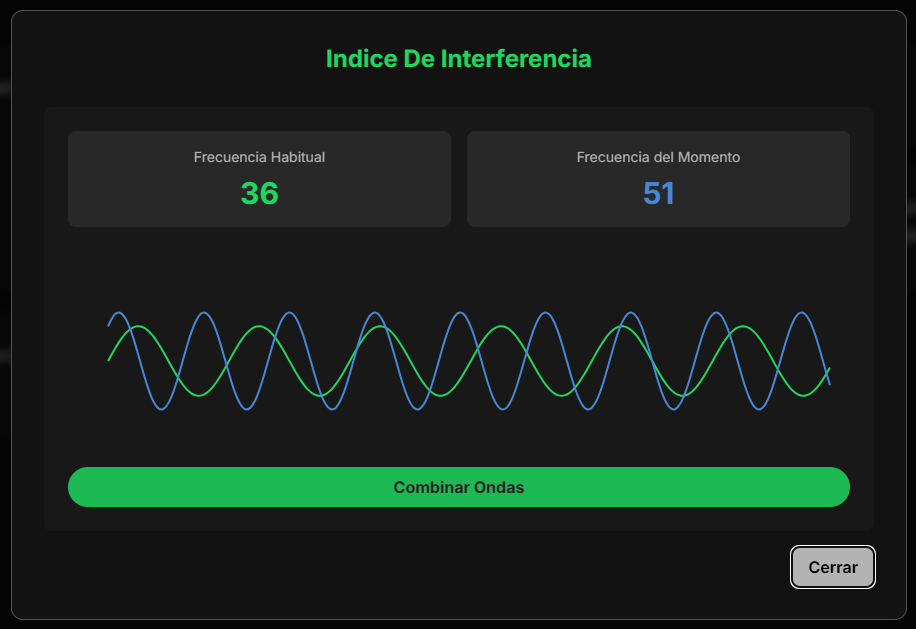
\includegraphics[width=\textwidth]{figures/capturas_ui/indice_de_interferencia_originales.png}
    \caption{Interfaz de la estadística \textit{Índice De Interferencia} (originales).}
    \label{fig:indice_de_interferencia_originales}
  \end{minipage}
  \begin{minipage}{0.47\textwidth}
    \centering
    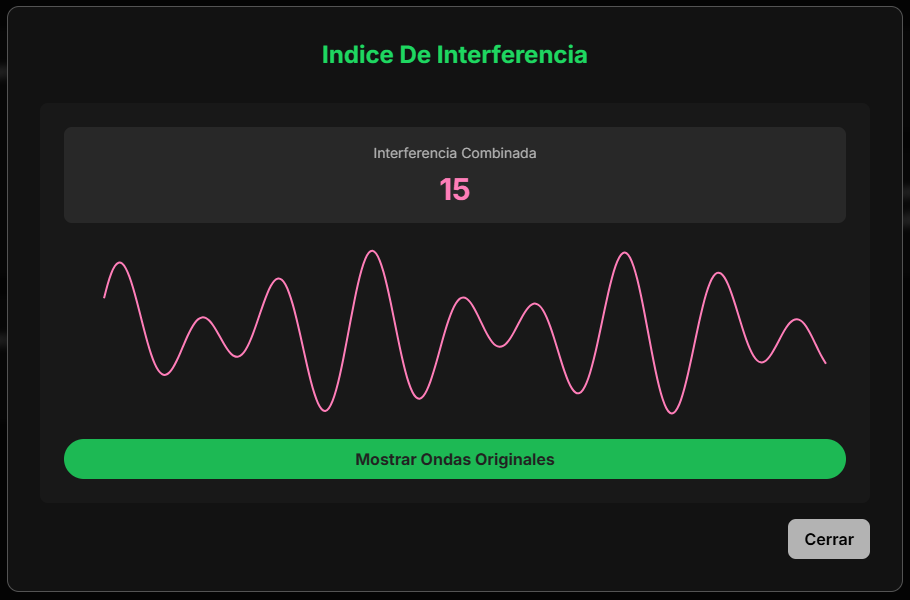
\includegraphics[width=\textwidth]{figures/capturas_ui/indice_de_interferencia_combinado.png}
    \caption{Interfaz de la estadística \textit{Índice De Interferencia} (combinados).}
    \label{fig:indice_de_interferencia_combinado}
  \end{minipage}
  \caption{Interfaz de la estadística \textit{Índice De Interferencia}, con las ondas originales y su forma combinada.}
  \label{fig:indice_de_interferencia}
\end{figure}

\section{Componentes Secundarios, de Carga y de Errores}

Además de los elementos presentados, también se han implementado algunos componentes secundarios para aportar más interactividad a la web y mejorar la experiencia al usuario.

\begin{figure}[H]
  \centering
  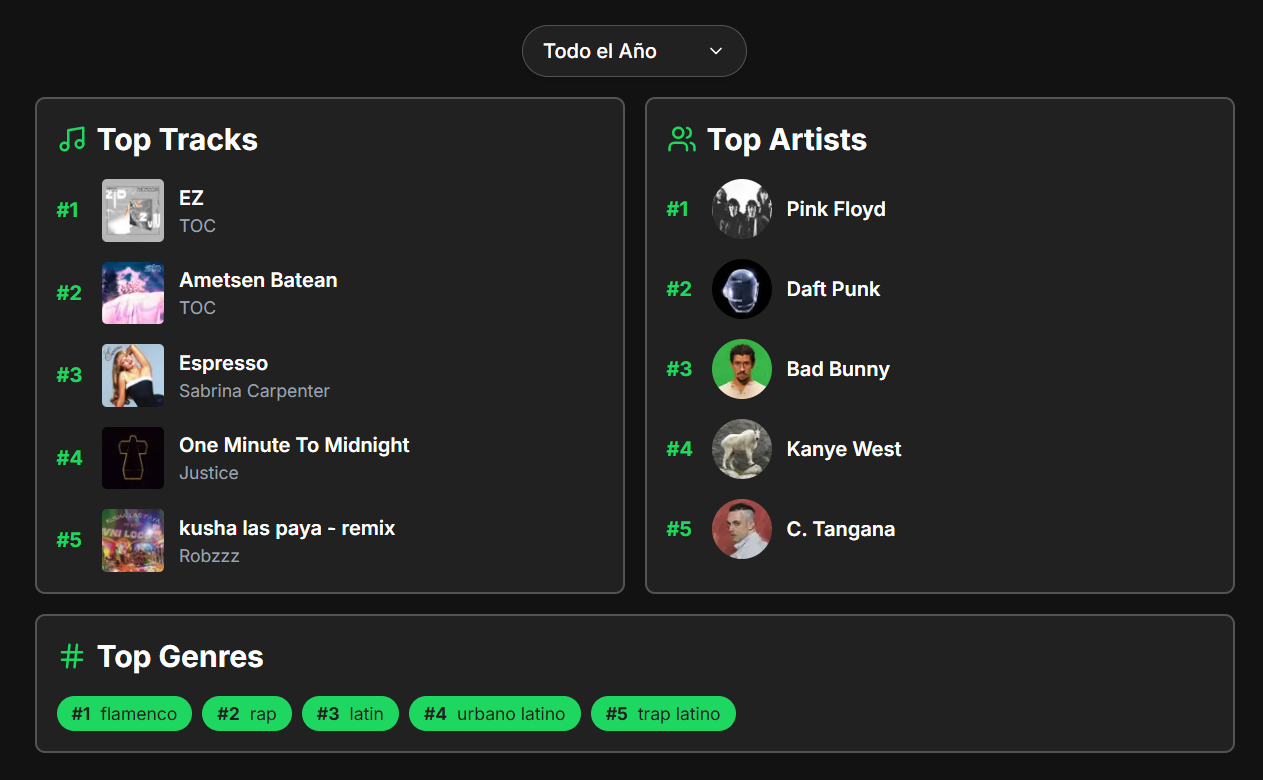
\includegraphics[width=0.75\textwidth]{figures/capturas_ui/tops_detalle.png}
  \caption{Detalle de los tres \textit{tops} junto con el selector de periodo de tiempo.}
  \label{fig:tops_detalle}
\end{figure}

\begin{figure}[H]
  \centering
  \vspace{-10pt}
  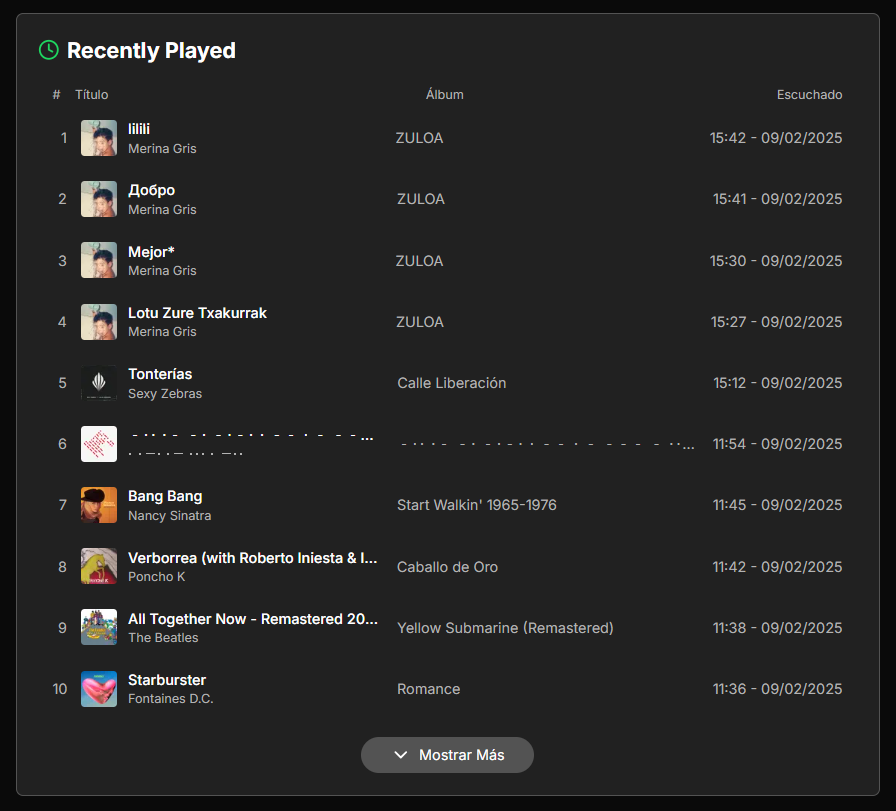
\includegraphics[width=0.75\textwidth]{figures/capturas_ui/recently_played.png}
  \caption{Detalle de \textit{Recently Played} con el botón para ampliar o contraer la lista.}
  \label{fig:recently_played}
\end{figure}

\begin{figure}[H]
  \centering
  \vspace{-10pt}
  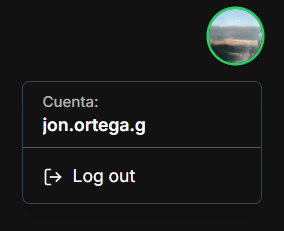
\includegraphics[width=0.4\textwidth]{figures/capturas_ui/user_action_panel.png}
  \caption{Panel del usuario con la opción de \textit{Log Out}.}
  \label{fig:user_action_panel}
\end{figure}

\begin{figure}[H]
  \centering
  \vspace{-10pt}
  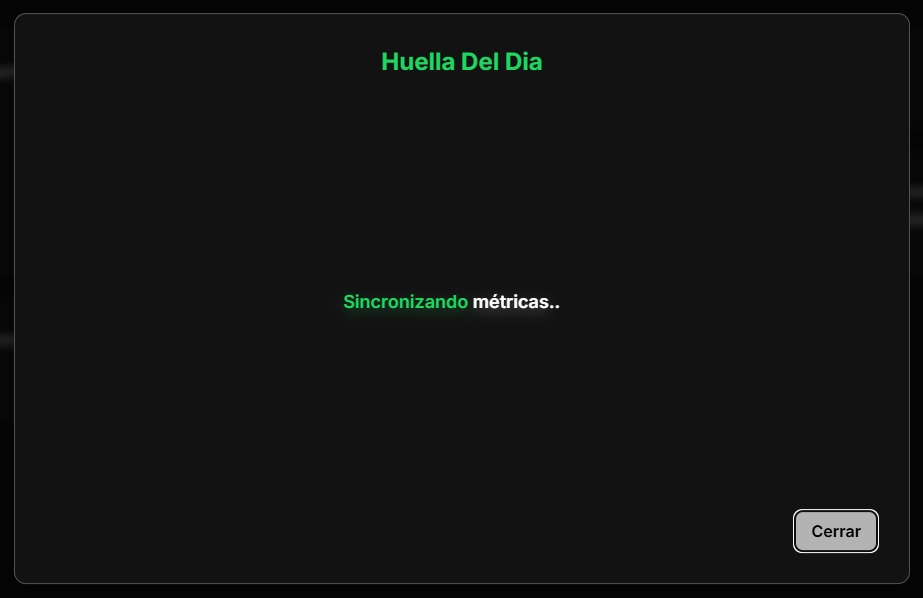
\includegraphics[width=0.75\textwidth]{figures/capturas_ui/pantalla_carga.png}
  \caption{Componente que se muestra mientras se cargan los datos de las estadísticas, con texto dinámico.}
  \label{fig:pantalla_carga}
\end{figure}

\begin{figure}[H]
  \centering
  \vspace{-10pt}
  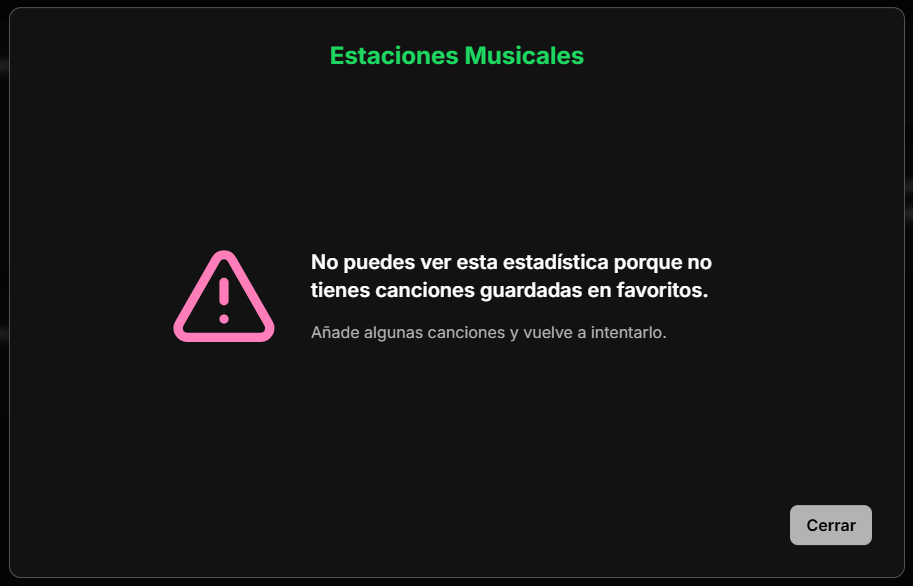
\includegraphics[width=0.75\textwidth]{figures/capturas_ui/error_no_favoritos.png}
  \caption{Componente de error que se muestra cuando el usuario no tiene ninguna canción guardada en su lista de favoritos.}
  \label{fig:error_no_favoritos}
\end{figure}

\begin{figure}[H]
  \centering
  \vspace{-10pt}
  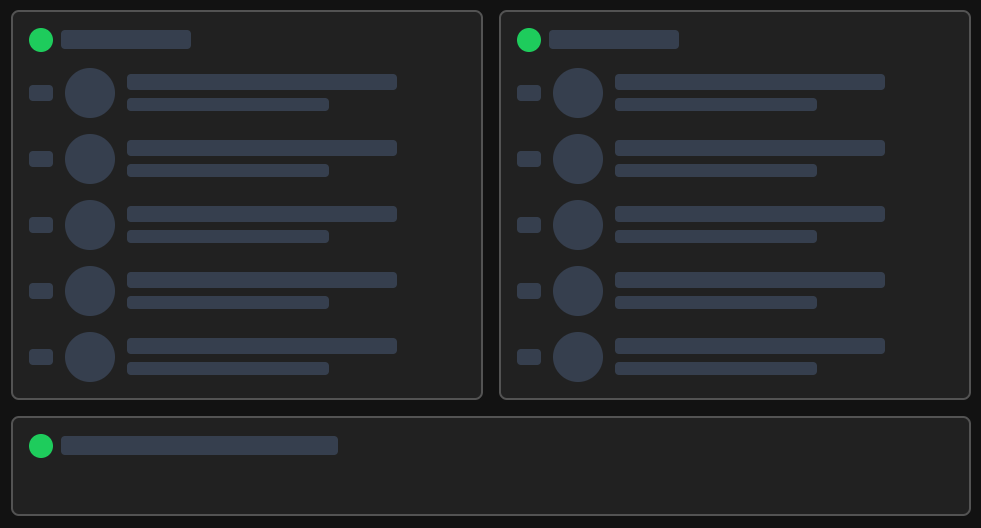
\includegraphics[width=0.8\textwidth]{figures/capturas_ui/skeletons.png}
  \caption{Componentes de \textit{loading} para los tres \textit{tops}.}
  \label{fig:skeletons}
\end{figure}

% * ANEXO B *

\chapter{Diagramas de Secuencia Adicionales} \label{ch:anexoB}

\begin{itemize}
  \item \textbf{Cerrar Sesión:} figura \ref{fig:ds_cerrar_sesion}
  \item \textbf{Ver Huella Del Día:} figura \ref{fig:ds_ver_huella_del_dia}
  \item \textbf{Ver Estaciones Musicales:} figura \ref{fig:ds_ver_estaciones_musicales}
  \item \textbf{Ver Tus Décadas:} figura \ref{fig:ds_ver_tus_decadas}
  \item \textbf{Ver Índice de Interferencia:} figura \ref{fig:ds_ver_indice_de_interferencia}
\end{itemize}

\begin{figure}[H]
  \centering
  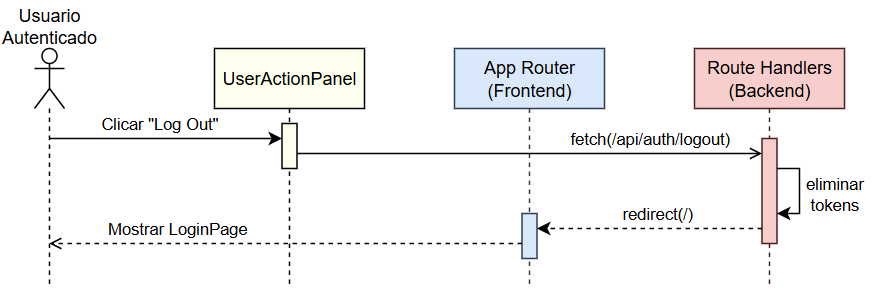
\includegraphics[width=0.85\textwidth]{figures/diagramas_secuencia/ds_cerrar_sesion.png}
  \caption{Diagrama de secuencia: \textbf{Cerrar Sesión}.}
  \label{fig:ds_cerrar_sesion}
\end{figure}

\begin{figure}[H]
  \centering
  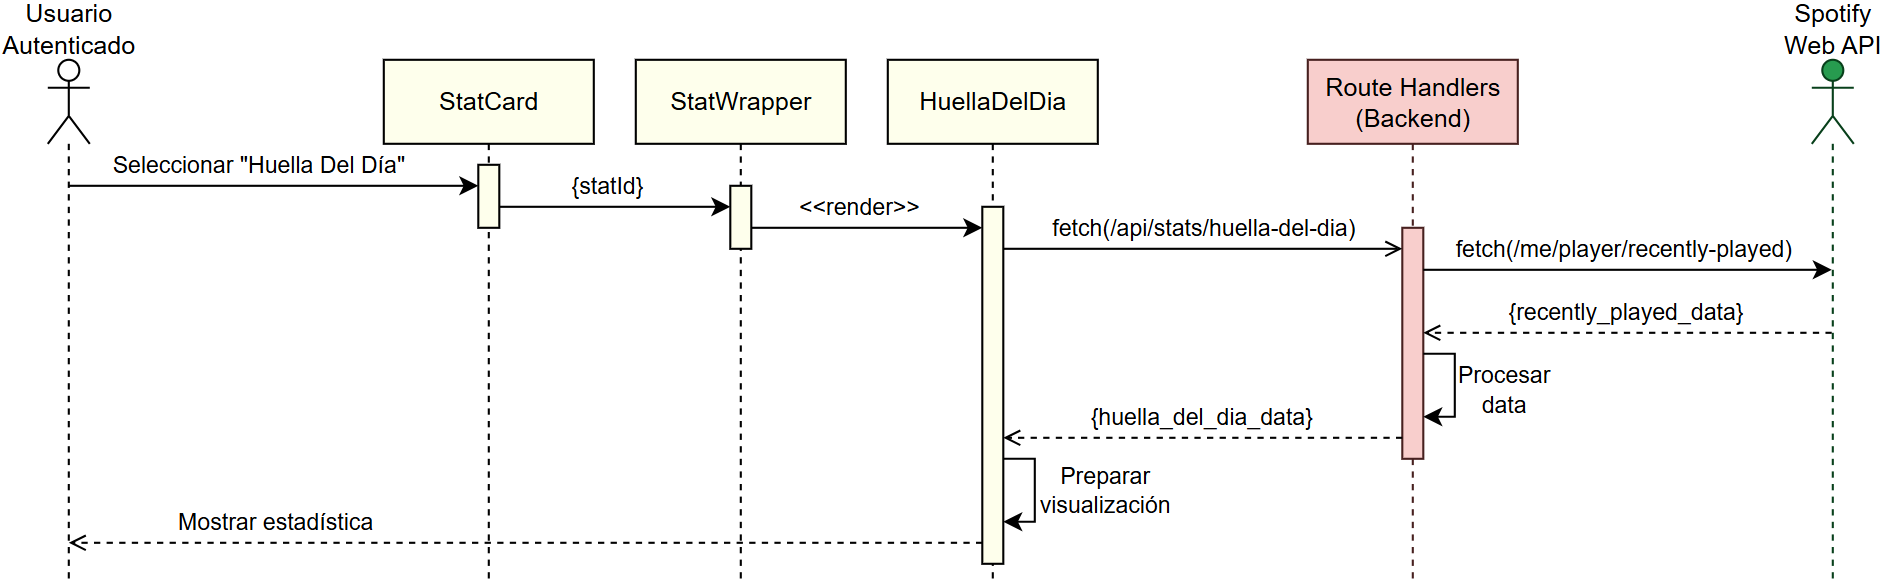
\includegraphics[width=\textwidth]{figures/diagramas_secuencia/ds_ver_huella_del_dia.png}
  \caption{Diagrama de secuencia: \textbf{Ver Huella Del Día}.}
  \label{fig:ds_ver_huella_del_dia}
\end{figure}

\begin{figure}[H]
  \centering
  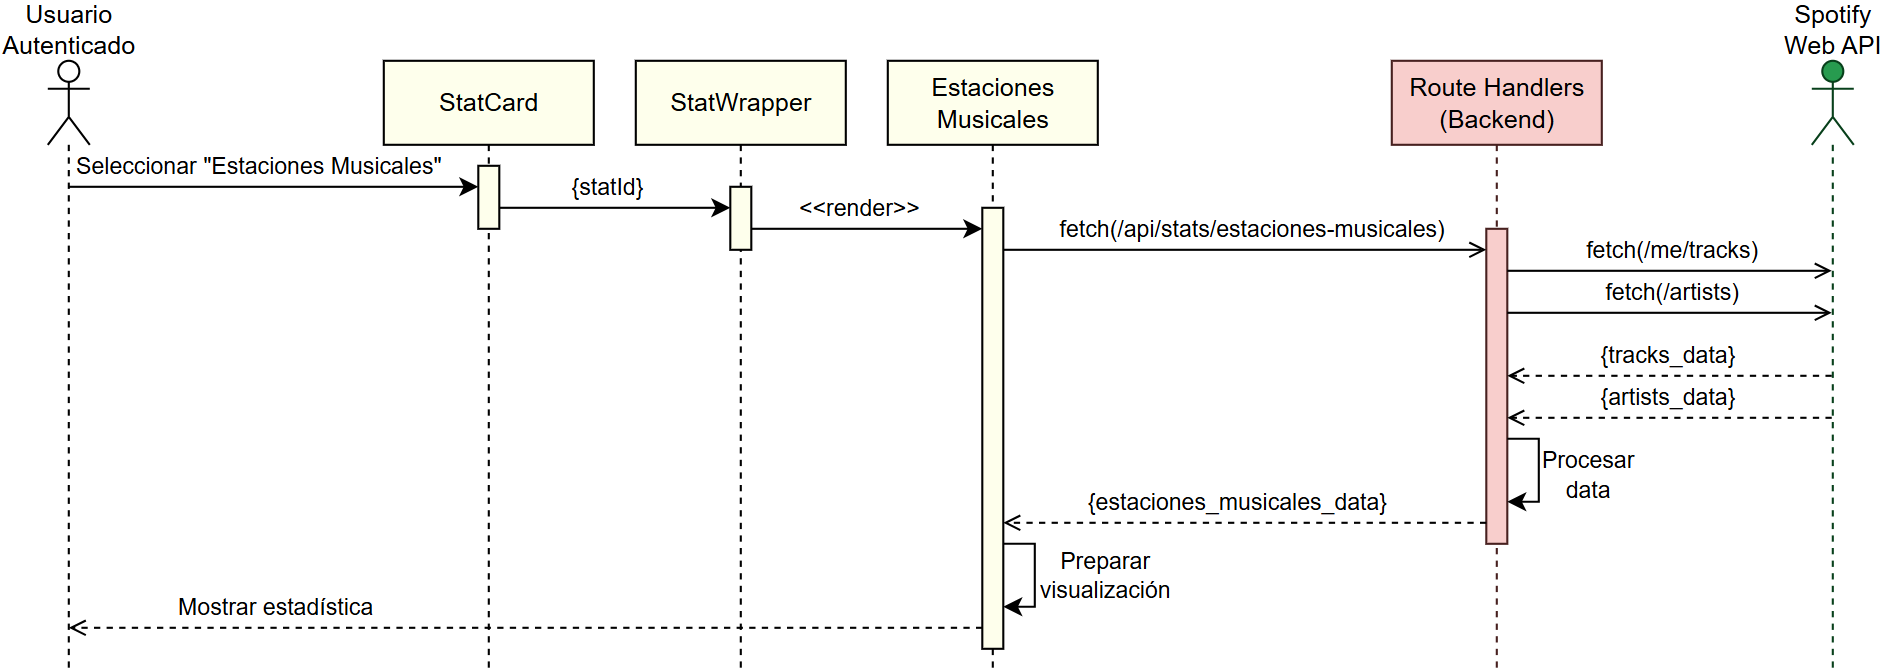
\includegraphics[width=\textwidth]{figures/diagramas_secuencia/ds_ver_estaciones_musicales.png}
  \caption{Diagrama de secuencia: \textbf{Ver Estaciones Musicales}.}
  \label{fig:ds_ver_estaciones_musicales}
\end{figure}

\begin{figure}[H]
  \centering
  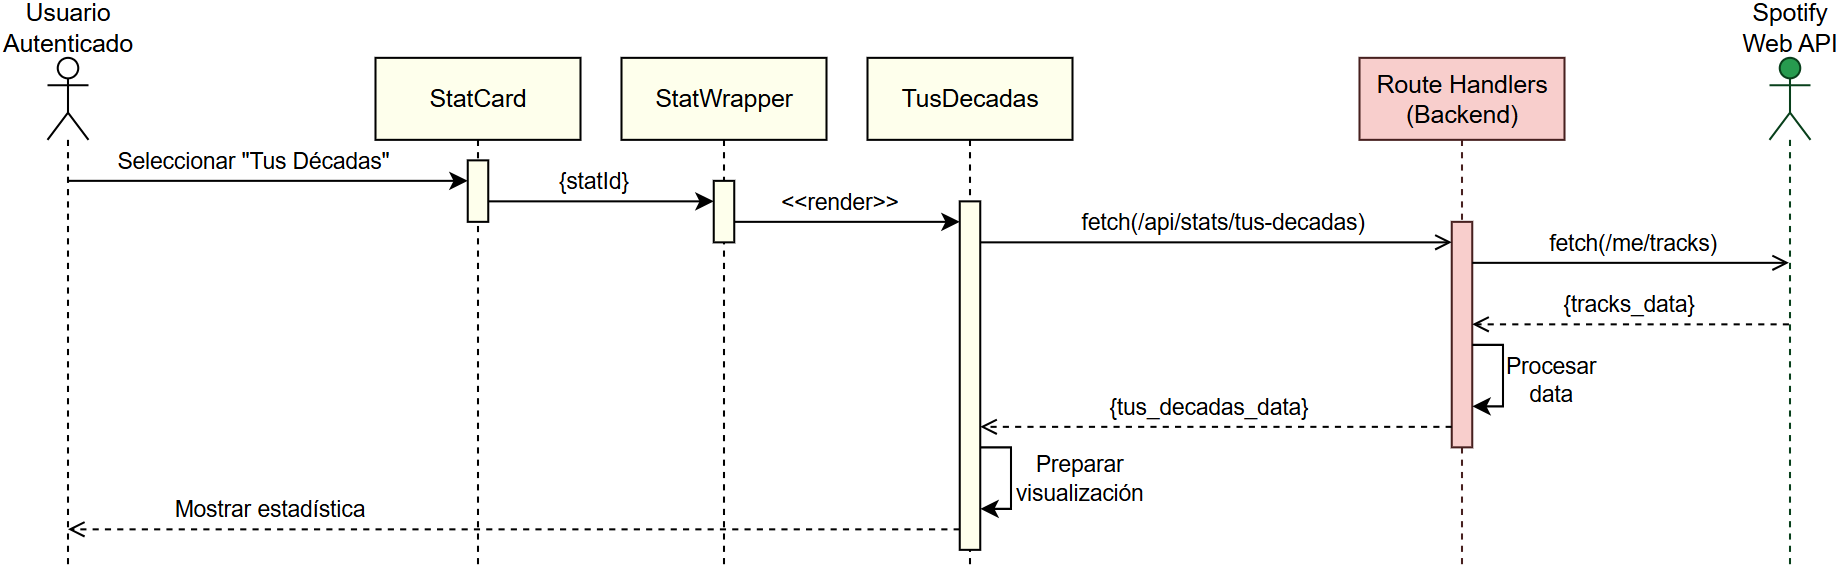
\includegraphics[width=\textwidth]{figures/diagramas_secuencia/ds_ver_tus_decadas.png}
  \caption{Diagrama de secuencia: \textbf{Ver Tus Décadas}.}
  \label{fig:ds_ver_tus_decadas}
\end{figure}

\begin{figure}[H]
  \centering
  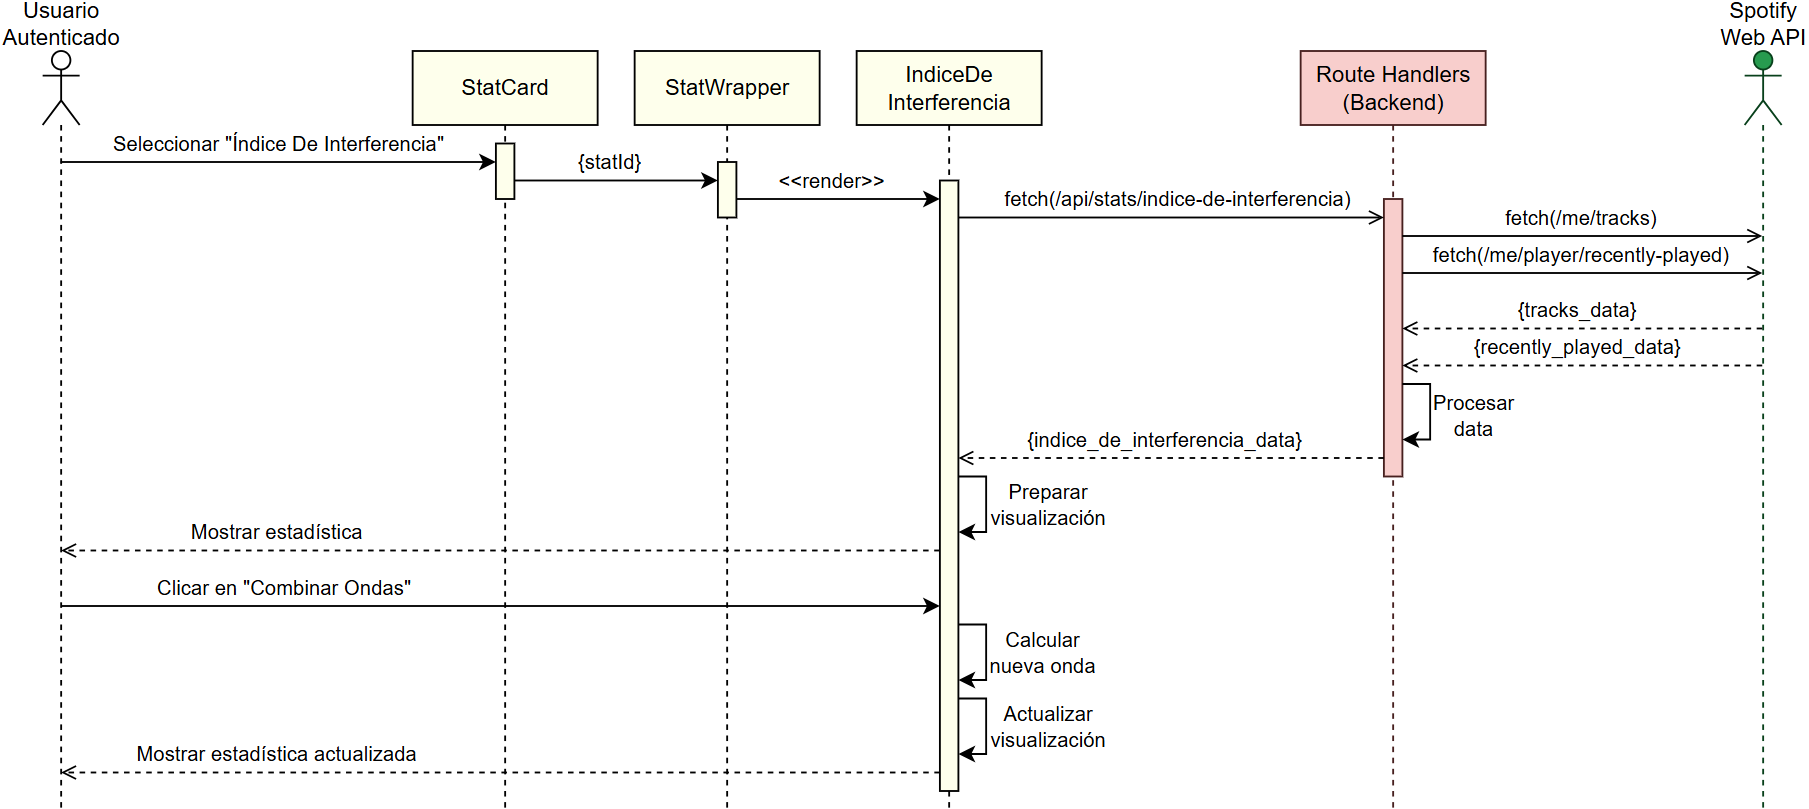
\includegraphics[width=\textwidth]{figures/diagramas_secuencia/ds_ver_indice_de_interferencia.png}
  \caption{Diagrama de secuencia: \textbf{Ver Índice De Interferencia}.}
  \label{fig:ds_ver_indice_de_interferencia}
\end{figure}

% * ANEXO C *

\chapter{Contenidos Relacionados con la Implementación} \label{ch:anexoC}

\section*{Fichero .env.local}

\begin{ifalgorithm}[H]
  \begin{lstlisting}[language=bash]
    # ID del cliente registrado en la API de Spotify
    SPOTIFY_CLIENT_ID="81af...642b"

    # Secreto del cliente registrado en la API de Spotify no compartir nunca
    SPOTIFY_CLIENT_SECRET="1207...393e"

    # URL del dominio donde se ejecuta la aplicacion en desarrollo, localhost
    DOMAIN_URL="http://localhost:3000"

    # URI de redireccion configurada en Spotify para la autenticacion OAuth
    SPOTIFY_REDIRECT_URI="http://localhost:3000/api/auth/callback"

    # URL utilizada por NextAuth para gestionar la autenticacion en la aplicacion
    NEXTAUTH_URL="http://localhost:3000/api/auth/callback"
    \end{lstlisting}
  \caption{Variables de entrono necesarios en el fichero \texttt{.env.local}.}
  \label{alg:variables_entorno}
\end{ifalgorithm}

\section*{Figura del Panel de Monitoreo de Spotify}

\begin{figure}[H]
  \centering
  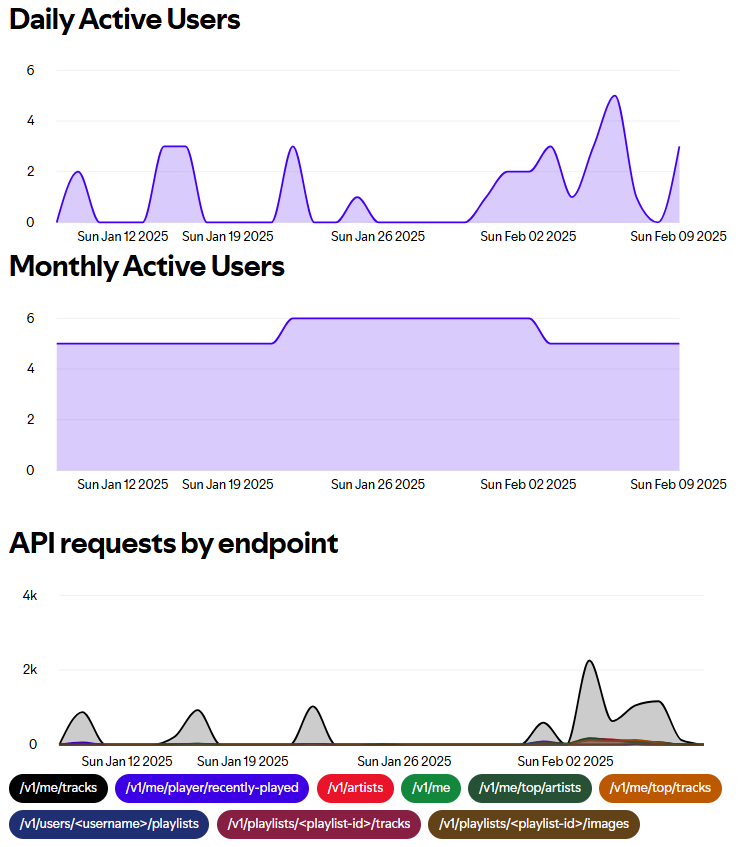
\includegraphics[width=0.75\textwidth]{figures/registro_spotify/dashboard_spotify.png}
  \caption{Panel de monitoreo de la actividad de la aplicación registrada.}
  \label{fig:dashboard_spotify}
\end{figure}

\section*{Definición del Hook Personalizado useFetch}

\begin{ifalgorithm}[H]
  \begin{lstlisting}
    import { useEffect, useState } from "react";

    interface UseFetchResult<T> {
      data: T | null;
      loading: boolean;
      error: string | null;
    }

    export function useFetch<T>(url: string): UseFetchResult<T> {
      const [data, setData] = useState<T | null>(null);
      const [loading, setLoading] = useState(true);
      const [error, setError] = useState<string | null>(null);

      useEffect(() => {
        const controller = new AbortController();
        const signal = controller.signal;
        let isAborted = false;

        console.log("=== INICIO DE FETCH, setLoading(true) ===");
        setLoading(true);
        setData(null);
        setError(null);

        fetch(url, { credentials: "include", signal })
          .then((response) => {
            if (!response.ok) throw new Error("Failed to fetch data");
            return response.json() as Promise<T>;
          })
          .then((result) => {
            if (!isAborted) setData(result);
          })
          .catch((err) => {
            if (err.name !== "AbortError") {
              console.error("Error fetching data:", err);
              if (!isAborted) setError("Error al cargar los datos. Por favor, intentalo de nuevo mas tarde.");
            } else {
              console.log("=== FETCH ABORTADO ===");
            }
          })
          .finally(() => {
            if (!isAborted) {
              console.log("=== FIN DE FETCH, setLoading(false) ===");
              setLoading(false);
            }
          });

        return () => {
          console.log("=== ABORTANDO FETCH ===");
          isAborted = true;
          controller.abort();
        };
      }, [url]);

      return { data, loading, error };
    }
    \end{lstlisting}
  \caption{Definición del \textit{hook} personalizado \texttt{useFetch} para la obtención de datos de la API con gestión de estado y abortos de petición.}
  \label{alg:use_fetch}
\end{ifalgorithm}

\section*{Código de los Componentes Home y Stats}

\begin{ifalgorithm}[H]
  \begin{lstlisting}
    export default async function Home({
      searchParams,
    }: {
      searchParams: Promise<Record<string, string | string[] | undefined>>;
    }) {
      const resolvedSearchParams = await searchParams;

      const timeRange = Array.isArray(resolvedSearchParams.time_range)
        ? resolvedSearchParams.time_range[0]
        : resolvedSearchParams.time_range || "short_term";

      return (
        <main className='min-h-screen relative'>
          <section className='bg-spotify-black'>
            <div className='max-w-5xl mx-auto px-4 md:px-8 py-8'>
              <h1 className='text-4xl md:text-5xl font-bold mb-12 text-center bg-gradient-to-r from-spotify-green to-spotify-blue bg-clip-text text-transparent'>
                Tus Spotify Tops
              </h1>
              <Suspense fallback={<UserProfileSkeleton />}>
                <UserProfile />
              </Suspense>
              <div className='flex justify-center mt-8'>
                <TimeRangeSelector />
              </div>
              <div className='grid grid-cols-1 md:grid-cols-2 gap-4'>
                <Suspense fallback={<TrackArtistSkeleton count={5} />}>
                  <TopTracks timeRange={timeRange} />
                </Suspense>
                <Suspense fallback={<TrackArtistSkeleton count={5} />}>
                  <TopArtists timeRange={timeRange} />
                </Suspense>
                <div className='md:col-span-2'>
                  <Suspense fallback={<GenreSkeleton count={5} />}>
                    <TopGenres timeRange={timeRange} />
                  </Suspense>
                </div>
              </div>
            </div>
          </section>
          <section className='bg-[#0A0A0A]'>
            <div className='max-w-5xl mx-auto px-4 md:px-8 py-12'>
              <RecentlyPlayed />
            </div>
          </section>
        </main>
      );
    }
    \end{lstlisting}
  \caption{Definición del componente \texttt{Home}, encargado de renderizar la página principal con las estadísticas de usuario en Spotify.}
  \label{alg:home_component}
\end{ifalgorithm}

\begin{ifalgorithm}[H]
  \begin{lstlisting}
    "use client";

    import { useState } from "react";
    import StatsGrid from "@/components/StatsGrid";
    import StatWrapper from "@/components/StatWrapper";

    // Define the type for a single stat item
    type StatItem = {
      id: string;
      title: string;
      iconName: keyof typeof import("lucide-react");
      className?: string;
    };

    // Define the stats array with the correct types
    const stats: StatItem[] = [
      {
        id: "hall-of-fame",
        title: "Hall of Fame",
        iconName: "Award",
        className: "md:col-span-2 lg:col-span-2 lg:row-span-2",
      },
      { id: "tus-decadas", title: "Tus Decadas", iconName: "Rewind", className: "md:col-span-1 lg:col-span-2" },
      {
        id: "huella-del-dia",
        title: "Huella Del Dia",
        iconName: "Fingerprint",
      },
      { id: "estaciones-musicales", title: "Estaciones Musicales", iconName: "SunSnow" },

      {
        id: "la-bitacora",
        title: "La Bitacora",
        iconName: "BookMarked",
        className: "md:col-span-2 lg:col-span-2",
      },
      { id: "indice-de-interferencia", title: "indice de Interferencia", iconName: "AudioWaveform" },
    ];

    export default function Stats() {
      const [activeStat, setActiveStat] = useState<string | null>(null);
      const [isModalOpen, setIsModalOpen] = useState(false);

      const handleStatClick = (statId: string) => {
        setActiveStat(statId);
        setIsModalOpen(true);
      };

      const handleCloseModal = () => {
        setActiveStat(null);
        setIsModalOpen(false);
      };

      return (
        <main className='bg-spotify-black min-h-screen'>
          <div className='max-w-7xl mx-auto px-4 sm:px-6 lg:px-8 py-12'>
            <h1 className='text-4xl md:text-5xl font-bold mb-12 text-center bg-gradient-to-r from-spotify-green to-spotify-blue bg-clip-text text-transparent'>
              Estadisticas Avanzadas
            </h1>
            <StatsGrid stats={stats} onStatClick={handleStatClick} />
          </div>
          <StatWrapper activeStat={activeStat} isOpen={isModalOpen} onClose={handleCloseModal} />
        </main>
      );
    }
    \end{lstlisting}
  \caption{Definición del componente \texttt{Stats}, encargado de gestionar y renderizar la interfaz de las estadísticas avanzadas.}
  \label{alg:stats_component}
\end{ifalgorithm}

\section*{Código del Componente StatWrapper}

\begin{ifalgorithm}[H]
  \begin{lstlisting}
    "use client";

    import { Dialog, DialogContent, DialogHeader, DialogTitle } from "@/components/ui/dialog";
    import dynamic from "next/dynamic";

    const statComponents = {
      "hall-of-fame": dynamic(() => import("@/components/stats/HallOfFame")),
      "estaciones-musicales": dynamic(() => import("@/components/stats/EstacionesMusicales")),
      "huella-del-dia": dynamic(() => import("@/components/stats/HuellaDelDia")),
      "la-bitacora": dynamic(() => import("@/components/stats/LaBitacora")),
      "tus-decadas": dynamic(() => import("@/components/stats/TusDecadas")),
      "indice-de-interferencia": dynamic(() => import("@/components/stats/IndiceDeInterferencia")),
    };

    interface StatWrapperProps {
      activeStat: string | null;
      isOpen: boolean;
      onClose: () => void;
    }

    export default function StatWrapper({ activeStat, isOpen, onClose }: StatWrapperProps) {
      const getStatComponent = (statId: string | null) => {
        if (!statId || !(statId in statComponents)) {
          return (
            <div className='text-sm text-spotify-gray-100'>
              Selecciona una estadistica valida para ver los detalles.
            </div>
          );
        }
        const DynamicComponent = statComponents[statId as keyof typeof statComponents];
        return <DynamicComponent />;
      };

      return (
        <Dialog open={isOpen} onOpenChange={(open) => !open && onClose()}>
          <DialogContent
            className={`${
              activeStat === "tus-decadas"
                ? "w-[90vw] max-w-7xl"
                : "w-[95vw] max-w-4xl"
            } min-h-[60vh] max-h-[90vh] overflow-y-auto p-8 flex flex-col`}
          >
            <DialogHeader>
              <DialogTitle className='text-2xl font-bold text-spotify-green'>
                {activeStat
                  ? activeStat
                      .split("-")
                      .map((word) => word.charAt(0).toUpperCase() + word.slice(1))
                      .join(" ")
                  : "Estadistica"}
              </DialogTitle>
            </DialogHeader>
            <div className='flex-1 flex items-center justify-center py-4'>
              <div className='w-full mx-auto'>{getStatComponent(activeStat)}</div>
            </div>
            <div className='mt-auto text-right'>
              <button
                onClick={onClose}
                className='px-4 py-2 bg-spotify-gray-100 text-black font-semibold rounded-lg hover:bg-spotify-green/90'
              >
                Cerrar
              </button>
            </div>
          </DialogContent>
        </Dialog>
      );
    }
    \end{lstlisting}
  \caption{Definición del componente \texttt{StatWrapper}, encargado de gestionar la visualización dinámica de estadísticas en un modal.}
  \label{alg:stat_wrapper}
\end{ifalgorithm}

\section*{Código Completo del Middleware}

\begin{ifalgorithm}[H]
  \begin{lstlisting}
    import { NextResponse } from "next/server";
    import type { NextRequest } from "next/server";
    import { renovarAccessToken } from "@/lib/spotify";

    export async function middleware(req: NextRequest) {
      const access_token = req.cookies.get("access_token");
      const refresh_token = req.cookies.get("refresh_token");

      // Caso 1: Si no hay ni access_token ni refresh_token, redirir al login
      if (!access_token && !refresh_token) {
        console.log("No hay tokens, redirigiendo al login...");
        return NextResponse.redirect(new URL("/", req.url));
      }

      // Caso 2: Si hay un refresh_token pero no un access_token, renovar el token
      if (!access_token && refresh_token) {
        console.log("No hay access_token, renovando...");
        const new_tokens = await renovarAccessToken(refresh_token.value);

        if (!new_tokens) {
          return NextResponse.redirect(new URL("/", req.url));
        }

        const res = NextResponse.next();

        res.cookies.set("access_token", new_tokens.access_token, {
          httpOnly: true,
          secure: process.env.NODE_ENV === "production",
          path: "/",
          maxAge: new_tokens.expires_in, // 1 hora
        });

        if (new_tokens.refresh_token) {
          res.cookies.set("refresh_token", new_tokens.refresh_token, {
            httpOnly: true,
            secure: process.env.NODE_ENV === "production",
            path: "/",
            maxAge: 60 * 60 * 24, // 1 dia
          });
        }

        return res;
      }

      // Caso 3: Si hay un access_token, dejar que la peticion continue
      return NextResponse.next();
    }

    // Rutas protegidas
    export const config = {
      matcher: ["/home/:path*", "/stats/:path*"],
    };
    \end{lstlisting}
  \caption{Middleware global en Next.js para la gestión y renovación de tokens de autenticación.}
  \label{alg:middleware}
\end{ifalgorithm}

\begin{ifalgorithm}[H]
  \begin{lstlisting}
    export async function renovarAccessToken(refresh_token: string) {
      const clientId = process.env.SPOTIFY_CLIENT_ID!;
      const clientSecret = process.env.SPOTIFY_CLIENT_SECRET!;
      const auth_header = Buffer.from(`${clientId}:${clientSecret}`).toString("base64");

      try {
        const response = await fetch("https://accounts.spotify.com/api/token", {
          method: "POST",
          headers: {
            "Content-Type": "application/x-www-form-urlencoded",
            Authorization: `Basic ${auth_header}`,
          },
          body: new URLSearchParams({
            grant_type: "refresh_token",
            refresh_token: refresh_token,
          }),
        });

        if (!response.ok) {
          console.error("Error al renovar el token:", await response.text());
          return null;
        }

        const data = await response.json();
        console.log("Access token renovado con exito");
        console.log("Nuevos tokens:\n", data);

        return {
          ...data,
          refresh_token: data.refresh_token || refresh_token,
        };
      } catch (error) {
        console.error("Error durante la renovacion del access token:", error);
        return null;
      }
    }
    \end{lstlisting}
  \caption{Función para la renovación del \texttt{access\_token} utilizando el \texttt{refresh\_token} en la API de Spotify.}
  \label{alg:renovar_access_token}
\end{ifalgorithm}

\section*{Función de Optimización de Imagen en Hall Of Fame}

\begin{ifalgorithm}[H]
  \begin{lstlisting}
    const optimizeImage = async (canvas: HTMLCanvasElement, maxSize: number): Promise<string> => {
      let quality = 0.9;
      let imageBase64: string;
      let size: number;

      do {
        imageBase64 = canvas.toDataURL("image/jpeg", quality).split(",")[1];
        size = Math.round((imageBase64.length * 0.75) / 1024);
        console.log(`Trying quality: ${quality.toFixed(2)}, size: ${size}KB`);
        quality -= 0.1;
      } while (size > maxSize && quality > 0.1);

      if (size > maxSize) {
        // If still too large, reduce dimensions
        const scaledCanvas = document.createElement("canvas");
        const ctx = scaledCanvas.getContext("2d");
        const scale = Math.sqrt(maxSize / size);

        scaledCanvas.width = canvas.width * scale;
        scaledCanvas.height = canvas.height * scale;

        if (ctx) {
          ctx.drawImage(canvas, 0, 0, scaledCanvas.width, scaledCanvas.height);
          imageBase64 = scaledCanvas.toDataURL("image/jpeg", 0.7).split(",")[1];
          size = Math.round((imageBase64.length * 0.75) / 1024);
          console.log(`Scaled down image. Final size: ${size}KB`);
        }
      }

      return imageBase64;
    };
    \end{lstlisting}
  \caption{Función \texttt{optimizeImage()} de optimización de imágenes con ajuste de calidad y escala.}
  \label{alg:optimize_image}
\end{ifalgorithm}

\section*{Función de Creación de SVGs en Estaciones Musicales}

\begin{ifalgorithm}[H]
  \begin{lstlisting}
    const calculatePath = (startAngle: number, endAngle: number, isHovered: boolean) => {
        const r = isHovered ? expandedRadius : radius;

        const x1 = r * Math.cos((startAngle * Math.PI) / 180);
        const y1 = r * Math.sin((startAngle * Math.PI) / 180);
        const x2 = r * Math.cos((endAngle * Math.PI) / 180);
        const y2 = r * Math.sin((endAngle * Math.PI) / 180);

        const largeArcFlag = endAngle - startAngle > 180 ? 1 : 0;

        return `
          M ${x1} ${y1}
          A ${r} ${r} 0 ${largeArcFlag} 1 ${x2} ${y2}
          L ${innerRadius * Math.cos((endAngle * Math.PI) / 180)} ${innerRadius * Math.sin((endAngle * Math.PI) / 180)}
          A ${innerRadius} ${innerRadius} 0 ${largeArcFlag} 0 ${
            innerRadius * Math.cos((startAngle * Math.PI) / 180)
          } ${innerRadius * Math.sin((startAngle * Math.PI) / 180)}
          Z
        `;
    };
    \end{lstlisting}
  \caption{Cálculo de la trayectoria de los segmentos en el gráfico de \textit{Estaciones Musicales}.}
  \label{alg:calculate_path}
\end{ifalgorithm}

\section*{Funciones de Movimiento y Zoom de Tus Décadas}

\begin{ifalgorithm}[H]
  \begin{lstlisting}
    <Stage
        width={stageWidth}
        height={600}
        draggable
        scaleX={scale}
        scaleY={scale}
        x={position.x}
        y={position.y}
        onWheel={handleWheel}
        onMouseDown={() => setCursorStyle("grabbing")} // Cambia a "grabbing"
        onMouseUp={() => setCursorStyle("grab")} // Vuelve a "grab"
        onMouseLeave={() => setCursorStyle("grab")} // Asegura que el cursor vuelva a "grab" al salir
        style={{
          cursor: cursorStyle, // Usa el estado del cursor
        }}
    >
    \end{lstlisting}
  \caption{Configuración del componente \texttt{Stage} en \textit{Tus Décadas}, permitiendo navegación y zoom dinámico.}
  \label{alg:stage_tus_decadas}
\end{ifalgorithm}

\begin{ifalgorithm}[H]
  \begin{lstlisting}
    const handleWheel = (e: any) => {
        e.evt.preventDefault();

        const scaleBy = 1.2;
        const stage = e.target.getStage();
        if (!stage) return;

        const oldScale = stage.scaleX();
        const mousePointTo = {
          x: stage.getPointerPosition()!.x / oldScale - stage.x() / oldScale,
          y: stage.getPointerPosition()!.y / oldScale - stage.y() / oldScale,
        };

        const newScale = e.evt.deltaY > 0 ? oldScale / scaleBy : oldScale * scaleBy;
        setScale(newScale);

        const newPos = {
          x: -(mousePointTo.x - stage.getPointerPosition()!.x / newScale) * newScale,
          y: -(mousePointTo.y - stage.getPointerPosition()!.y / newScale) * newScale,
        };

        setPosition(newPos);
    };
    \end{lstlisting}
  \caption{Manejo del evento de desplazamiento con la rueda del ratón en \textit{Tus Décadas} para aplicar zoom dinámico.}
  \label{alg:handle_wheel_tus_decadas}
\end{ifalgorithm}

\section*{Funciones de Generación de Ondas de Índice De Interferencia}

\begin{ifalgorithm}[H]
  \begin{lstlisting}
    const generateWaveData = (frequency: number, amplitude: number = 0.5, phase: number = 0) => {
        return Array.from({ length: 200 }, (_, i) => ({
          x: i,
          y: amplitude * Math.sin(((frequency / 25) * i * Math.PI) / 24 + phase),
        }));
    };
    \end{lstlisting}
  \caption{Generación de datos de onda sinusoidal en \textit{Índice de Interferencia} a partir de la frecuencia de escucha del usuario.}
  \label{alg:generate_wave_data}
\end{ifalgorithm}

\begin{ifalgorithm}[H]
  \begin{lstlisting}
    const drawWave = (data: { x: number; y: number }[], color: string, delay: number = 0, waveType: WaveType) => {
        const path = svg
          .append("path")
          .datum(data)
          .attr("fill", "none")
          .attr("stroke", color)
          .attr("stroke-width", 2)
          .attr("d", lineGenerator)
          .attr("opacity", 0)
          .attr("class", `wave-${waveType}`);

        const totalLength = path.node()?.getTotalLength() || 0;

        path
          .attr("stroke-dasharray", totalLength + " " + totalLength)
          .attr("stroke-dashoffset", totalLength)
          .transition()
          .duration(1000)
          .delay(delay)
          .attr("opacity", 1)
          .transition()
          .duration(1500)
          .attr("stroke-dashoffset", 0);

        return path;
    };
    \end{lstlisting}
  \caption{Función \texttt{drawWave()} para dibujar ondas sinusoidales animadas en \textit{Índice de Interferencia} utilizando D3.js.}
  \label{alg:draw_wave}
\end{ifalgorithm}


% * ANEXO D *

\chapter{Información del Backend de las Estadísticas Avanzadas} \label{ch:anexoD}

\section{Información del Backend del Hall Of Fame} \label{sec:backend_hall_of_fame}

\begin{ifalgorithm}[H]
  \begin{lstlisting}
    // * GET /api/stats/hall-of-fame
    1. Obtener access_token de las cookies.
    2. Si no hay access_token, devolver error 401.
    3. Realizar una peticion a la API de Spotify para obtener las 16 canciones mas escuchadas a largo plazo.
    4. Si la peticion no es exitosa, devolver error 500.
    5. Extraer la informacion relevante de cada cancion:
       - URL de la imagen del album
       - Nombre de la cancion
       - Nombre del artista principal
    6. Estructurar los datos en un array de objetos Album.
    7. Enviar la respuesta en formato JSON con los datos procesados.

    // * POST /api/stats/hall-of-fame
    1. Obtener access_token de las cookies.
    2. Si no hay access_token, devolver error 401.
    3. Obtener la imagen de portada desde el cuerpo de la peticion.
    4. Realizar una peticion a la API de Spotify para obtener las 16 canciones mas escuchadas.
    5. Extraer las URIs de las canciones.
    6. Obtener el perfil del usuario y su userId.
    7. Crear una nueva playlist privada llamada "Hall Of Fame".
    8. Extraer el playlistId de la respuesta.
    9. Anadir las canciones obtenidas a la playlist recien creada.
    10. Actualizar la imagen de portada de la playlist con la imagen proporcionada.
    11. Enviar respuesta en JSON con el playlistId creado si todo ha sido exitoso.
    \end{lstlisting}
  \caption{Pseudocódigo del procesamiento de datos en el endpoint Hall Of Fame.}
  \label{alg:hall_of_fame}
\end{ifalgorithm}

\begin{ifalgorithm}[H]
  \begin{lstlisting}
    {
      "title": "Hall of Fame",
      "albums": [
        {
          "albumArtUrl": "https://i.scdn.co/image/abc123",
          "track": "Bohemian Rhapsody",
          "artist": "Queen"
        },
        {
          "albumArtUrl": "https://i.scdn.co/image/xyz456",
          "track": "Billie Jean",
          "artist": "Michael Jackson"
        },
        ...
      ]
    }
    \end{lstlisting}
  \caption{Ejemplo de estructura de datos enviada en el endpoint Hall Of Fame.}
  \label{alg:hall_of_fame_response}
\end{ifalgorithm}

\section{Informacion del Backend de Estaciones Musicales} \label{sec:backend_estaciones_musicales}

\begin{ifalgorithm}[H]
  \begin{lstlisting}
    // * GET /api/stats/estaciones-musicales
    1. Obtener access_token de las cookies.
    2. Si no hay access_token, devolver error 401.
    3. Inicializar una estructura para almacenar los datos de artistas y generos por estacion.
    4. Obtener todos los tracks guardados por el usuario hasta un ano atras, recorriendo la API de Spotify con paginacion.
    5. Determinar la estacion correspondiente de cada track segun su fecha de agregado.
    6. Contar la frecuencia de aparicion de cada artista y almacenar sus IDs.
    7. Obtener datos de artistas en lotes de 50 desde la API de Spotify.
    8. Actualizar la informacion de cada artista con su imagen y contar los generos musicales asociados.
    9. Determinar el artista y genero mas representativos en cada estacion segun la frecuencia de aparicion.
    10. Estructurar los datos en un objeto JSON con la informacion obtenida.
    11. Enviar la respuesta en formato JSON con los datos procesados.
    \end{lstlisting}
  \caption{Pseudocodigo del procesamiento de datos en el endpoint Estaciones Musicales.}
  \label{alg:estaciones_musicales}
\end{ifalgorithm}

\begin{ifalgorithm}[H]
  \begin{lstlisting}
    {
      "invierno": {
        "artist": {
          "name": "Coldplay",
          "artistPicUrl": "https://i.scdn.co/image/coldplay123"
        },
        "genre": {
          "name": "Alternative Rock"
        }
      },
      "primavera": {
        "artist": {
          "name": "Dua Lipa",
          "artistPicUrl": "https://i.scdn.co/image/dualipa123"
        },
        "genre": {
          "name": "Pop"
        }
      },
      "verano": {
        "artist": {
          "name": "Bad Bunny",
          "artistPicUrl": "https://i.scdn.co/image/badbunny123"
        },
        "genre": {
          "name": "Reggaeton"
        }
      },
      "otono": {
        "artist": {
          "name": "The Beatles",
          "artistPicUrl": "https://i.scdn.co/image/beatles123"
        },
        "genre": {
          "name": "Rock"
        }
      }
    }
    \end{lstlisting}
  \caption{Ejemplo de estructura de datos enviada en el endpoint Estaciones Musicales.}
  \label{alg:estaciones_musicales_response}
\end{ifalgorithm}

\section{Información del Backend de Huella del Día} \label{sec:backend_huella_del_dia}

\begin{ifalgorithm}[H]
  \begin{lstlisting}
    // * GET /api/stats/huella-del-dia
    1. Obtener access_token de las cookies.
    2. Si no hay access_token, devolver error 401.
    3. Inicializar la URL base para obtener el historial de reproduccion reciente.
    4. Inicializar una lista para almacenar todas las canciones reproducidas.
    5. Realizar una peticion a la API de Spotify para obtener las ultimas 50 canciones reproducidas.
    6. Si la peticion es exitosa:
       a. Agregar las canciones obtenidas a la lista total.
       b. Verificar si hay mas paginas de resultados.
       c. Si hay mas paginas, actualizar la URL y repetir la peticion.
    7. Si la peticion falla, devolver error con el mensaje correspondiente.
    8. Inicializar un array de 24 posiciones para almacenar los minutos escuchados por cada hora del dia.
    9. Iterar sobre todas las canciones obtenidas y extraer:
       a. La hora en la que se reprodujo la cancion.
       b. Su duracion en minutos (limitada a un maximo de 60 por hora).
    10. Acumular el tiempo de reproduccion en la hora correspondiente dentro del array.
    11. Limitar cada posicion del array a un maximo de 60 minutos por hora.
    12. Enviar la respuesta en formato JSON con los datos procesados.
    \end{lstlisting}
  \caption{Pseudocodigo del procesamiento de datos en el endpoint Huella del Dia.}
  \label{alg:huella_del_dia}
\end{ifalgorithm}

\begin{ifalgorithm}[H]
  \begin{lstlisting}
    [5, 12, 25, 35, 50, 42, 30, 20, 15, 10, 8, 5, 3, 2, 1, 0, 0, 0, 5, 10, 20, 30, 40, 50]
    \end{lstlisting}
  \caption{Ejemplo de estructura de datos enviada en el endpoint Huella del Dia.}
  \label{alg:huella_del_dia_response}
\end{ifalgorithm}

\section{Información del Backend de La Bitácora} \label{sec:backend_la_bitacora}

\begin{ifalgorithm}[H]
  \begin{lstlisting}
    // * GET /api/stats/la-bitacora
    1. Obtener access_token de las cookies.
    2. Si no hay access_token, devolver error 401.
    3. Extraer los parametros de consulta (year y month) de la URL.
    4. Si la cache no esta inicializada:
       a. Obtener todas las canciones guardadas del usuario desde la API de Spotify.
       b. Extraer las fechas de guardado de cada cancion y estructurarlas en objetos con year, month y day.
       c. Agregar todas las canciones obtenidas a una lista total.
       d. Crear una estructura de almacenamiento:
          - Diccionario de anios con el total de canciones guardadas por cada anio.
          - Diccionario de meses por anio con el total de canciones guardadas por cada mes.
          - Diccionario de dias por anio-mes con el total de canciones guardadas por dia.
    5. Completar los periodos faltantes con valor 0:
       a. Rellenar los anio faltantes desde el primer hasta el ultimo.
       b. Rellenar los meses faltantes en cada anio.
       c. Rellenar los dias faltantes en cada mes considerando la cantidad de dias de cada mes.
    6. Si no se proporciona un anio en la consulta, devolver la estructura de datos por anio.
    7. Si se proporciona solo un anio, devolver la estructura de datos por mes para ese anio.
    8. Si se proporciona un anio y un mes, devolver la estructura de datos por dia para ese mes.
    9. Enviar la respuesta en formato JSON con los datos procesados.
    \end{lstlisting}
  \caption{Pseudocodigo del procesamiento de datos en el endpoint La Bitacora.}
  \label{alg:la_bitacora}
\end{ifalgorithm}

\begin{ifalgorithm}[H]
  \begin{lstlisting}
    {
      "2020": 150,
      "2021": 120,
      "2022": 180
    }
    \end{lstlisting}
  \caption{Ejemplo de estructura de datos enviada por año en el endpoint La Bitacora.}
  \label{alg:la_bitacora_response_year}
\end{ifalgorithm}

\begin{ifalgorithm}[H]
  \begin{lstlisting}
    {
      "2022-01": 15,
      "2022-02": 10,
      "2022-03": 20
    }
    \end{lstlisting}
  \caption{Ejemplo de estructura de datos enviada por mes en el endpoint La Bitacora.}
  \label{alg:la_bitacora_response_month}
\end{ifalgorithm}

\begin{ifalgorithm}[H]
  \begin{lstlisting}
    {
      "2022-03-01": 5,
      "2022-03-02": 3,
      "2022-03-03": 8
    }
    \end{lstlisting}
  \caption{Ejemplo de estructura de datos enviada por dia en el endpoint La Bitacora.}
  \label{alg:la_bitacora_response_day}
\end{ifalgorithm}

\section{Información del Backend de Tus Décadas} \label{sec:backend_tus_decadas}

\begin{ifalgorithm}[H]
  \begin{lstlisting}
    // * GET /api/stats/tus-decadas
    1. Obtener access_token de las cookies.
    2. Si no hay access_token, devolver error 401.
    3. Inicializar una lista para almacenar los albums procesados y un conjunto para evitar duplicados.
    4. Definir la URL inicial para la paginacion de las canciones guardadas en Spotify.
    5. Mientras haya una URL valida:
       a. Realizar una peticion a la API de Spotify para obtener los tracks guardados.
       b. Iterar sobre los tracks obtenidos:
          - Si el album ya ha sido procesado, omitirlo.
          - Extraer la imagen de mayor resolucion disponible.
          - Si no hay imagen disponible, omitir el track.
          - Extraer el anio de lanzamiento del album segun su precision de fecha.
          - Agregar la informacion del album procesado a la lista.
          - Registrar el album en el conjunto de albums procesados.
       c. Actualizar la URL con la siguiente pagina de resultados, si existe.
    6. Ordenar los tracks por anio de lanzamiento.
    7. Determinar el rango de decadas abarcadas por los datos:
       - Encontrar el anio minimo y redondearlo al inicio de la decada correspondiente.
       - Encontrar el anio maximo y redondearlo al final de la decada correspondiente.
    8. Construir una estructura de datos que agrupe los albums por anio.
    9. Rellenar los anios faltantes dentro del rango completo de decadas con listas vacias.
    10. Enviar la respuesta en formato JSON con los datos procesados.
    \end{lstlisting}
  \caption{Pseudocodigo del procesamiento de datos en el endpoint Tus Decadas.}
  \label{alg:tus_decadas}
\end{ifalgorithm}

\begin{ifalgorithm}[H]
  \begin{lstlisting}
    {
      "1970": [
        {
          "id": "album1",
          "albumPicUrl": "https://i.scdn.co/image/abc123",
          "year": 1970
        }
      ],
      "1980": [
        {
          "id": "album2",
          "albumPicUrl": "https://i.scdn.co/image/xyz456",
          "year": 1980
        },
        {
          "id": "album3",
          "albumPicUrl": "https://i.scdn.co/image/def789",
          "year": 1980
        }
      ],
      "1990": [],
      "2000": [
        {
          "id": "album4",
          "albumPicUrl": "https://i.scdn.co/image/ghi101",
          "year": 2000
        }
      ]
    }
    \end{lstlisting}
  \caption{Ejemplo de estructura de datos enviada en el endpoint Tus Decadas.}
  \label{alg:tus_decadas_response}
\end{ifalgorithm}

\section{Información del Backend de Índice de Interferencia} \label{sec:backend_indice_de_interferencia}

\begin{ifalgorithm}[H]
  \begin{lstlisting}
    // * GET /api/stats/indice-de-interferencia
    1. Obtener access_token de las cookies.
    2. Si no hay access_token, devolver error 401.

    // * Calcular el valor "normal" basado en canciones guardadas
    3. Definir un porcentaje del 20% de canciones a muestrear, con un minimo de 500 y un maximo de 1000 canciones.
    4. Realizar una peticion a la API de Spotify para obtener el total de canciones guardadas.
    5. Si el total de canciones guardadas es menor o igual a 500:
       a. Obtener todas las canciones paginando la API de Spotify.
    6. Si hay mas de 500 canciones:
       a. Generar offsets aleatorios para seleccionar una muestra representativa.
       b. Realizar peticiones a la API de Spotify usando estos offsets para obtener una muestra aleatoria.
    7. Calcular la popularidad media de las canciones obtenidas y redondear el resultado.

    // * Calcular el valor "actual" basado en reproducciones recientes
    8. Realizar una peticion a la API de Spotify para obtener las ultimas 50 canciones reproducidas.
    9. Calcular la popularidad media de estas canciones y redondear el resultado.

    // * Responder con los datos calculados
    10. Devolver un JSON con los valores "normal" y "actual".
    \end{lstlisting}
  \caption{Pseudocodigo del procesamiento de datos en el endpoint Indice de Interferencia.}
  \label{alg:indice_interferencia}
\end{ifalgorithm}

\begin{ifalgorithm}[H]
  \begin{lstlisting}
    {
      "normal": 75,
      "actual": 62
    }
    \end{lstlisting}
  \caption{Ejemplo de estructura de datos enviada en el endpoint Indice de Interferencia.}
  \label{alg:indice_interferencia_response}
\end{ifalgorithm}


\chapter{Tablas de Tests Realizados} \label{ch:anexoE}

\section{Pruebas de Componentes}

\begin{longtable}{|p{5cm}|p{9cm}|}
  \caption{Pruebas realizadas en los componentes \textit{de Next.js}.} \label{tab:pruebas_componentes}                           \\

  \hline
  \rowcolor[HTML]{E6B8CE}
  \textbf{\textcolor{white}{Componente}}          & \textbf{\textcolor{white}{Test}}                                             \\ \hline
  \endfirsthead

  \hline
  \rowcolor[HTML]{E6B8CE}
  \textbf{\textcolor{white}{Componente}}          & \textbf{\textcolor{white}{Test}}                                             \\ \hline
  \endhead

  \hline \multicolumn{2}{|r|}{\textit{Continúa en la siguiente página}}                                                          \\ \hline
  \endfoot

  \hline
  \endlastfoot

  \multirow{5}{*}{\texttt{Footer}}                & se renderiza correctamente                                                   \\ \cline{2-2}
                                                  & contiene enlaces de redes sociales                                           \\ \cline{2-2}
                                                  & el modal de Política de Privacidad está cerrado al inicio                    \\ \cline{2-2}
                                                  & abre el modal de Política de Privacidad al hacer clic                        \\ \cline{2-2}
                                                  & cierra el modal al hacer clic en 'Cerrar'                                    \\ \hline

  \multirow{3}{*}{\texttt{Loading}}               & se renderiza correctamente con una frase inicial                             \\ \cline{2-2}
                                                  & actualiza la frase cada 3 segundos                                           \\ \cline{2-2}
                                                  & muestra los puntos de carga dinámicamente                                    \\ \hline

  \multirow{2}{*}{\texttt{LoginPage}}             & renderiza el heading principal                                               \\ \cline{2-2}
                                                  & renderiza el botón de Sign In                                                \\ \hline

  \multirow{5}{*}{\texttt{Navbar}}                & renderiza correctamente la barra de navegación                               \\ \cline{2-2}
                                                  & muestra el enlace Home como activo cuando la ruta es /home                   \\ \cline{2-2}
                                                  & muestra el enlace Stats como activo cuando la ruta es /stats                 \\ \cline{2-2}
                                                  & muestra el enlace Home como inactivo cuando la ruta NO es /home              \\ \cline{2-2}
                                                  & pasa correctamente el usuario al UserActionPanel                             \\ \hline

  \multirow{2}{*}{\texttt{NoFavorites}}           & se renderiza correctamente con el mensaje adecuado                           \\ \cline{2-2}
                                                  & muestra el icono de advertencia                                              \\ \hline

  \multirow{6}{*}{\texttt{RecentlyPlayed}}        & se renderiza correctamente con el título 'Recently Played'                   \\ \cline{2-2}
                                                  & muestra el mensaje de carga cuando está cargando                             \\ \cline{2-2}
                                                  & muestra un mensaje de error cuando ocurre un error                           \\ \cline{2-2}
                                                  & muestra canciones cuando hay datos disponibles                               \\ \cline{2-2}
                                                  & muestra un mensaje cuando no hay canciones recientes                         \\ \cline{2-2}
                                                  & cambia entre mostrar más y mostrar menos correctamente                       \\ \hline

  \multirow{3}{*}{\texttt{Stats Page}}            & renderiza StatsGrid con los elementos esperados                              \\ \cline{2-2}
                                                  & abre el modal con la estadística seleccionada al hacer clic en un stat       \\ \cline{2-2}
                                                  & cierra el modal cuando se hace clic en el botón de cierre                    \\ \hline

  \multirow{4}{*}{\texttt{StatCard}}              & se renderiza correctamente con el título                                     \\ \cline{2-2}
                                                  & renderiza el icono correctamente                                             \\ \cline{2-2}
                                                  & llama a onClick con el statId correcto cuando se hace clic                   \\ \cline{2-2}
                                                  & aplica la clase className correctamente                                      \\ \hline

  \multirow{3}{*}{\texttt{StatsGrid}}             & renderiza StatsGrid con los elementos esperados                              \\ \cline{2-2}
                                                  & abre el modal con la estadística seleccionada al hacer clic en un stat       \\ \cline{2-2}
                                                  & cierra el modal cuando se hace clic en el botón de cierre                    \\ \hline

  \multirow{3}{*}{\texttt{StatWrapper}}           & se renderiza correctamente                                                   \\ \cline{2-2}
                                                  & llama a onStatClick con el id correcto cuando se hace clic en un StatCard    \\ \cline{2-2}
                                                  & maneja correctamente una lista vacía de stats sin errores                    \\ \hline

  \multirow{10}{*}{\texttt{TimeRangeSelector}}    & no se renderiza cuando isOpen es false                                       \\ \cline{2-2}
                                                  & se renderiza correctamente cuando isOpen es true                             \\ \cline{2-2}
                                                  & muestra el título correcto basado en `activeStat`                            \\ \cline{2-2}
                                                  & renderiza el componente dinámico correcto                                    \\ \cline{2-2}
                                                  & muestra un mensaje cuando `activeStat` es inválido                           \\ \cline{2-2}
                                                  & cierra el modal al hacer clic en el botón de cierre                          \\ \cline{2-2}
                                                  & desmonta correctamente el contenido cuando el modal se cierra                \\ \cline{2-2}
                                                  & muestra mensaje de error cuando se selecciona una estadística no válida      \\ \cline{2-2}
                                                  & muestra el componente de Hall of Fame cuando se selecciona                   \\ \cline{2-2}
                                                  & muestra el componente de Huella Del Día cuando se selecciona                 \\ \hline

  \multirow{10}{*}{\texttt{UserActionPanel}}      & muestra el valor seleccionado correctamente                                  \\ \cline{2-2}
                                                  & abre el menú al hacer clic en el botón y muestra las opciones                \\ \cline{2-2}
                                                  & cierra el menú al hacer clic fuera                                           \\ \cline{2-2}
                                                  & actualiza el parámetro de la URL al seleccionar una opción                   \\ \cline{2-2}
                                                  & cierra el menú al seleccionar una opción                                     \\ \cline{2-2}
                                                  & renderiza correctamente la imagen y el nombre del usuario                    \\ \cline{2-2}
                                                  & abre y cierra el panel de usuario al hacer clic                              \\ \cline{2-2}
                                                  & cierra el panel al hacer clic fuera                                          \\ \cline{2-2}
                                                  & ejecuta el logout y redirige al usuario a la página principal                \\ \cline{2-2}
                                                  & muestra un error en la consola si el logout falla                            \\ \hline

  \multirow{4}{*}{\texttt{HuellaDelDia}}          & las etiquetas del eje X van de '00:00' a '23:00'                             \\ \cline{2-2}
                                                  & el gráfico recibe los datos correctos cuando useFetch devuelve datos válidos \\ \cline{2-2}
                                                  & el gráfico muestra un punto destacado en la hora con más minutos escuchados  \\ \cline{2-2}
                                                  & el texto debajo del gráfico muestra correctamente la hora con más escuchas   \\ \hline

  \multirow{1}{*}{\texttt{IndiceDeInterferencia}} & IndiceDeInterferencia se renderiza sin errores                               \\ \hline

  \multirow{3}{*}{\texttt{TusDecadas}}            & se renderiza sin errores                                                     \\ \cline{2-2}
                                                  & muestra mensaje de error cuando la API falla                                 \\ \cline{2-2}
                                                  & muestra correctamente las etiquetas de las décadas según los datos de la API \\ \hline
\end{longtable}

\section{Pruebas de Utilidades}

\begin{longtable}{|p{5cm}|p{9cm}|}
  \caption{Pruebas realizadas en las utilidades del proyecto.} \label{tab:pruebas_utilidades}                                \\

  \hline
  \rowcolor[HTML]{E6B8CE}
  \textbf{\textcolor{white}{Utilidad}}       & \textbf{\textcolor{white}{Test}}                                              \\ \hline
  \endfirsthead

  \hline
  \rowcolor[HTML]{E6B8CE}
  \textbf{\textcolor{white}{Utilidad}}       & \textbf{\textcolor{white}{Test}}                                              \\ \hline
  \endhead

  \hline \multicolumn{2}{|r|}{\textit{Continúa en la siguiente página}}                                                      \\ \hline
  \endfoot

  \hline
  \endlastfoot

  \multirow{4}{*}{\texttt{fetchTopArtists}}  & devuelve una lista de artistas correctamente cuando la API responde con éxito \\ \cline{2-2}
                                             & devuelve un array vacío si no se proporciona access\_token                    \\ \cline{2-2}
                                             & devuelve un array vacío si la respuesta de la API no es exitosa               \\ \cline{2-2}
                                             & devuelve un array vacío si ocurre un error en la petición                     \\ \hline

  \multirow{4}{*}{\texttt{fetchTopGenres}}   & devuelve una lista de géneros correctamente cuando la API responde con éxito  \\ \cline{2-2}
                                             & devuelve un array vacío si no se proporciona access\_token                    \\ \cline{2-2}
                                             & devuelve un array vacío si la respuesta de la API no es exitosa               \\ \cline{2-2}
                                             & devuelve un array vacío si ocurre un error en la petición                     \\ \hline

  \multirow{2}{*}{\texttt{fetchTopTracks}}   & devuelve una lista de tracks correctamente                                    \\ \cline{2-2}
                                             & maneja errores correctamente                                                  \\ \hline


  \multirow{3}{*}{\texttt{fetchUserProfile}} & devuelve error si no hay access\_token                                        \\ \cline{2-2}
                                             & maneja errores cuando la API responde con fallo                               \\ \cline{2-2}
                                             & devuelve el perfil del usuario cuando la API responde correctamente           \\ \hline


  \multirow{4}{*}{\texttt{useFetch Hook}}    & devuelve datos correctamente cuando la API responde con éxito                 \\ \cline{2-2}
                                             & maneja correctamente un error en la petición (error de red)                   \\ \cline{2-2}
                                             & devuelve un error si la respuesta de la API no es exitosa                     \\ \cline{2-2}
                                             & cancela la petición cuando el componente se desmonta                          \\ \hline
\end{longtable}

\section{Pruebas de Endpoints del Backend}

\begin{longtable}{|p{5cm}|p{9cm}|}
  \caption{Pruebas realizadas en los endpoints del backend.} \label{tab:pruebas_route_handlers}                                                    \\

  \hline
  \rowcolor[HTML]{E6B8CE}
  \textbf{\textcolor{white}{Endpoint}}                  & \textbf{\textcolor{white}{Test}}                                                         \\ \hline
  \endfirsthead

  \hline
  \rowcolor[HTML]{E6B8CE}
  \textbf{\textcolor{white}{Endpoint}}                  & \textbf{\textcolor{white}{Test}}                                                         \\ \hline
  \endhead

  \hline \multicolumn{2}{|r|}{\textit{Continúa en la siguiente página}}                                                                            \\ \hline
  \endfoot

  \hline
  \endlastfoot

  \multirow{2}{*}{\texttt{/auth/callback}}              & debe redirigir con error si faltan los parámetros \texttt{code} y \texttt{state}         \\ \cline{2-2}
                                                        & debe redirigir con error si el estado no coincide con la cookie                          \\ \hline
  \multirow{4}{*}{\texttt{/auth/login}}                 & debe redirigir a la página de autenticación de Spotify con los parámetros correctos      \\ \cline{2-2}
                                                        & debe establecer la cookie \texttt{spotify\_auth\_state} correctamente                    \\ \cline{2-2}
                                                        & debe generar un \textit{state} aleatorio en cada llamada                                 \\ \cline{2-2}
                                                        & debe generar un \textit{state} válido en formato hex                                     \\ \hline
  \multirow{2}{*}{\texttt{/auth/logout}}                & debe redirigir al usuario a \texttt{/} después del logout                                \\ \cline{2-2}
                                                        & debe eliminar las cookies \texttt{access\_token} y \texttt{refresh\_token} correctamente \\ \hline
  \multirow{4}{*}{\texttt{/home/recently-played}}       & debe devolver 401 si no se proporciona el token de acceso                                \\ \cline{2-2}
                                                        & debe obtener correctamente las canciones recientemente reproducidas                      \\ \cline{2-2}
                                                        & debe manejar correctamente respuestas sin imágenes o nombres de álbum                    \\ \cline{2-2}
                                                        & debe devolver error 500 si la API de Spotify falla                                       \\ \hline
  \multirow{5}{*}{\texttt{/home/top-artists}}           & debe devolver 401 si no se proporciona el token de acceso                                \\ \cline{2-2}
                                                        & debe devolver 401 si el token de acceso es inválido                                      \\ \cline{2-2}
                                                        & debe obtener los top 5 artistas correctamente                                            \\ \cline{2-2}
                                                        & debe manejar correctamente respuestas malformadas                                        \\ \cline{2-2}
                                                        & debe devolver error 500 si la API de Spotify falla                                       \\ \hline
  \multirow{5}{*}{\texttt{/home/top-genres}}            & debe devolver 401 si no se proporciona el token de acceso                                \\ \cline{2-2}
                                                        & debe devolver 401 si el token de acceso es inválido                                      \\ \cline{2-2}
                                                        & debe obtener los top 5 géneros correctamente                                             \\ \cline{2-2}
                                                        & debe manejar correctamente artistas sin géneros                                          \\ \cline{2-2}
                                                        & debe devolver error 500 si la API de Spotify falla                                       \\ \hline
  \multirow{5}{*}{\texttt{/home/top-tracks}}            & debe devolver 401 si no se proporciona el token de acceso                                \\ \cline{2-2}
                                                        & debe devolver 401 si el token de acceso es inválido                                      \\ \cline{2-2}
                                                        & debe obtener los top 5 tracks correctamente                                              \\ \cline{2-2}
                                                        & debe manejar correctamente respuestas malformadas                                        \\ \cline{2-2}
                                                        & debe devolver error 500 si la API de Spotify falla                                       \\ \hline
  \multirow{5}{*}{\texttt{/home/user-profile}}          & debe devolver 401 si no se proporciona el token de acceso                                \\ \cline{2-2}
                                                        & debe devolver 401 si el token de acceso es inválido                                      \\ \cline{2-2}
                                                        & debe obtener el perfil de usuario correctamente                                          \\ \cline{2-2}
                                                        & debe manejar correctamente usuarios sin nombre, email o imagen                           \\ \cline{2-2}
                                                        & debe devolver error 500 si la API de Spotify falla                                       \\ \hline
  \multirow{4}{*}{\texttt{/stats/estaciones-musicales}} & debe devolver 401 si no se proporciona el token de acceso                                \\ \cline{2-2}
                                                        & debe devolver artistas y géneros destacados por estación                                 \\ \cline{2-2}
                                                        & debe manejar correctamente la paginación de la API de Spotify                            \\ \cline{2-2}
                                                        & debe devolver error 500 si la API de Spotify falla                                       \\ \hline
  \multirow{3}{*}{\texttt{/stats/huella-del-dia}}       & debe devolver 401 si no se proporciona el token de acceso                                \\ \cline{2-2}
                                                        & debe devolver un array de 24 posiciones con valores numéricos                            \\ \cline{2-2}
                                                        & debe devolver un error 500 si la API de Spotify falla                                    \\ \hline
  \multirow{4}{*}{\texttt{/stats/tus-decadas}}          & debe devolver 401 si no se proporciona el token de acceso                                \\ \cline{2-2}
                                                        & debe devolver los tracks correctamente agrupados por década                              \\ \cline{2-2}
                                                        & debe manejar correctamente cuando no hay canciones guardadas                             \\ \cline{2-2}
                                                        & debe devolver error 500 si la API de Spotify falla                                       \\ \hline
\end{longtable}

